\documentclass[12pt,
	english,			% idioma adicional para hifenização
	french,				% idioma adicional para hifenização
	spanish,			% idioma adicional para hifenização
	brazil,				% o último idioma é o principal do documento
	]{article}

%% Language and font encodings
\usepackage[brazil]{babel}
\usepackage[utf8x]{inputenc}
\usepackage[T1]{fontenc}
\usepackage{indentfirst}
\usepackage{float}

%% Sets page size and margins
\usepackage[a4paper,top=3cm,bottom=2cm,left=3cm,right=3cm,marginparwidth=1.75cm]{geometry}

%% Useful packages
\usepackage{amsmath}
\usepackage{graphicx}
\usepackage[colorinlistoftodos]{todonotes}
\usepackage[colorlinks=true, allcolors=blue]{hyperref}
\usepackage{url}
\usepackage{listings}

\usepackage{xcolor}

\definecolor{codegreen}{rgb}{0,0.6,0}
\definecolor{codegray}{rgb}{0.5,0.5,0.5}
\definecolor{codepurple}{rgb}{0.58,0,0.82}
\definecolor{backcolour}{rgb}{0.95,0.95,0.92}

\lstdefinestyle{mystyle}{
    backgroundcolor=\color{backcolour},   
    commentstyle=\color{codegreen},
    keywordstyle=\color{magenta},
    numberstyle=\tiny\color{codegray},
    stringstyle=\color{codepurple},
    %%basicstyle=\ttfamily\footnotesize,
    basicstyle=\scriptsize,
    breakatwhitespace=false,         
    breaklines=true,                 
    captionpos=b,                    
    keepspaces=true,                 
    numbers=left,                    
    numbersep=5pt,                  
    showspaces=false,                
    showstringspaces=false,
    showtabs=false,                  
    tabsize=2
}

\lstset{style=mystyle}

%% Document Header
\title{Laboratório 03 - CNN\\
\Large{Aprendizado de Máquina - INFO7004}\\
\Large{Prof. Luiz Eduardo S. Oliveira, Ph.D}}

\author{Discente: Marc Queiroz}
\date{08 de setembro de 2020}

%% Document Begin
\begin{document}
\maketitle

%\begin{abstract}

% Seu resumo do relatório, resumo não é introdução! Por exemplo, o excerto abaixo foi extraído do relatório de alunos do 1s2017, note que ele resume as atividades desenvolvidas e apresentadas no relatório, porém não faz uma introdução exagerada ao assunto abordado.
%"\textit{Calculamos a partir da montagem de circuitos RC e RLC a resistência interna do osciloscópio, bem como os valores de capacitância dos componentes utilizados. Analisamos as curvas dos circuitos passa-altas, passa-baixas e passa banda, juntamente com seus respectivos diagramas de bode, comparando-as com curvas esperadas fornecidas na literatura sobre o assunto. Utilizando um método baseado em assíndotas, estimamos valores para as frequências de ressonância e de corte, comparando-os com valores experimentais e teóricos}"

%\end{abstract}

\section{Introdução}

A prática do laboratório 3 apresenta uma base de dados de imagens com escritas manuais com os meses do ano. A tarefa consiste em analisar a implementação e treinamento de CNNs e também a geração de imagens utilizando a técnica de \textit{data augmentation} para classificação dessas imagens.

Os códigos fontes utilizados nesse laboratório e a versão mais atual desse relatório pode ser encontrado no GitHub, \url{https://github.com/marc-queiroz/ml_lab3/}.

O trabalho está subdivido em seções, as primeiras apresentam as CNNs do trabalho. Uma explicação dos métodos de augumentação também faz parte do trabalho, em seção própria. Apresentadas as CNNs e técnicas utilizas segue-se para os experimentos, neles são apresentadas os testes com e sem augumentação para as duas redes. Em seção própria, é apresentado os resultados dos experimentos. Também foi escolhido duas redes pré-treinadas da ImageNet, Inception v4, VGG16 para realizar os experimentos de (Transfer Learning/Fine-Tuning). Chegando a parte final, com a extração de características utilizando a rede pré-treinada Inception v4. Com a última seção mostrando os resultados do teste com o classificador SVM com kernel radial. 

\section{LeNet-5}

A rede LeNet-5 é uma rede convolucional de 7 camadas, descrita no artigo \cite{Lecun98gradient-basedlearning}. O treinamento dessa rede é feita através de uma rede neural que aplica convoluções e filtros consecutivos, para assim encontrar os melhores pesos de acordo com sua base de treinamento.

O propósito inicial da LeNet-5 foi identificar dígitos escritos manualmente, figura \ref{fig:image_lenet5}. Para implementar essa CNN utilizou-se a API Keras, que permite uma representação de fácil leitura e manutenção. O código da rede pode ser encontrado na listagem \ref{code:modelo_lenet}.

\newpage

\begin{figure}[!ht]
  \centering
  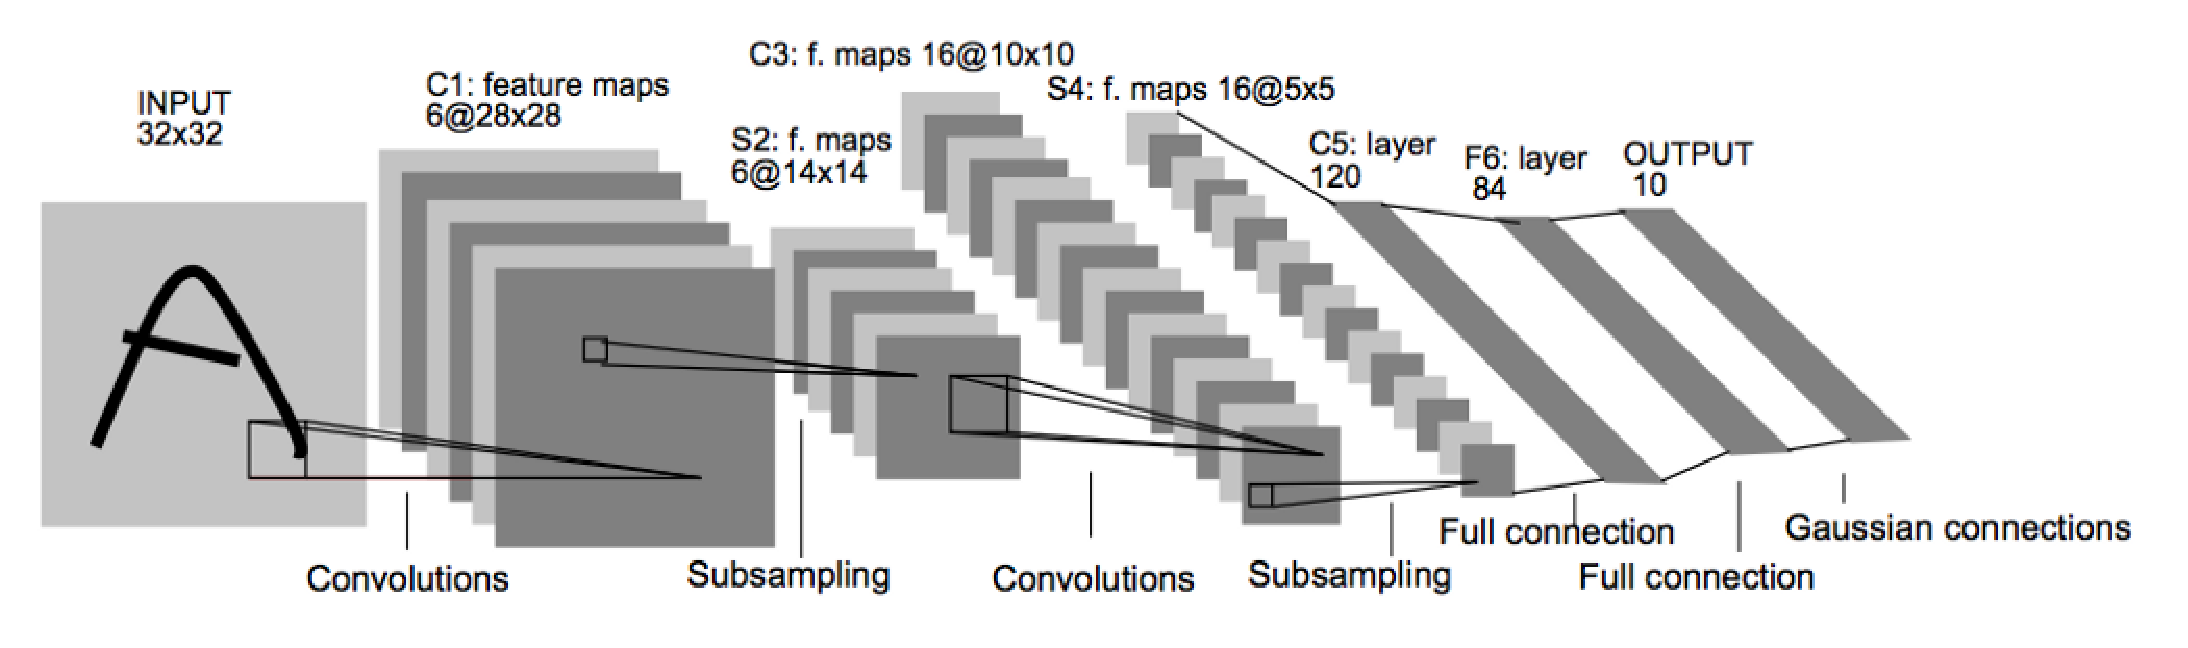
\includegraphics[width=35em]{images/lenet5.pdf}
  \caption{As 7 camadas do modelo LeNet-5\cite{Lecun98gradient-basedlearning}}
  \label{fig:image_lenet5}
\end{figure}

\begin{lstlisting}[caption={LeNet-5 implementado em Keras},captionpos=b,frame=single,label={code:modelo_lenet}, language=Python][ht]
model = keras.Sequential()
model.add(layers.Conv2D(filters=6, kernel_size=(3, 3), activation='relu', input_shape=(32,32,1)))
model.add(layers.AveragePooling2D())
model.add(layers.Conv2D(filters=16, kernel_size=(3, 3), activation='relu'))
model.add(layers.AveragePooling2D())
model.add(layers.Flatten())
model.add(layers.Dense(units=120, activation='relu'))
model.add(layers.Dense(units=84, activation='relu'))
model.add(layers.Dense(units=12, activation = 'softmax'))
\end{lstlisting}

A rede é composta por 7 camadas, sendo elas:
\begin{enumerate}
  \item C1 convolucional (tamanho de saída: 28x28x6)
  \item S2 pooling (agrupamento) (tamanho de saída: 14x14x6)
  \item C3 convolucional (tamanho de saída: 10x10x6)
  \item S4 pooling (agrupamento) (tamanho de saída: 5x5x16)
  \item C5 classificação (tamanho de saída: 120)
  \item F6 classificação (tamanho de saída: 84)
  \item OUTPUT (tamanho de saída: 12)
\end{enumerate}

Observa-se que o tamanho do vetor OUTPUT tem a quantidade de categorias sendo classificadas, 12 meses.

\section{Outra CNN}

A CNN escolhida foi adaptada do autor, Francois Lemarchand, no site, \url{https://www.kaggle.com/frlemarchand/simple-cnn-using-keras}, refere-se a um experimento para reconhecimento de cactus em imagens. Seguindo o desenvolvimento sugerido para redes convolucionais o autor procurou criar uma rede convolucional para resolver um problema binário. 

Para utilizar essa rede nos experimentos, a sua camada de saída foi alterada para 12 classes, ao invés de 2, originais, listagem \ref{code:modelo_personalizado}.

\begin{lstlisting}[caption={CNN escolhida},captionpos=b,frame=single,label={code:modelo_personalizado}, language=Python]
dropout_dense_layer = 0.6

model = Sequential()
model.add(Conv2D(32, (3, 3), input_shape=input_shape))
model.add(BatchNormalization())
model.add(Activation('relu'))
model.add(Conv2D(32, (3, 3)))
model.add(BatchNormalization())
model.add(Activation('relu'))
model.add(Conv2D(32, (3, 3)))
model.add(BatchNormalization())
model.add(Activation('relu'))
model.add(MaxPooling2D(pool_size=(2, 2)))

model.add(Conv2D(64, (3, 3)))
model.add(BatchNormalization())
model.add(Activation('relu'))
model.add(Conv2D(64, (3, 3)))
model.add(BatchNormalization())
model.add(Activation('relu'))
model.add(Conv2D(64, (3, 3)))
model.add(BatchNormalization())
model.add(Activation('relu'))
model.add(MaxPooling2D(pool_size=(2, 2)))

model.add(Conv2D(128, (3, 3)))
model.add(BatchNormalization())
model.add(Activation('relu'))

model.add(Flatten())
model.add(Dense(1024))
model.add(Activation('relu'))
model.add(Dropout(dropout_dense_layer))

model.add(Dense(256))
model.add(Activation('relu'))
model.add(Dropout(dropout_dense_layer))

model.add(Dense(12))
model.add(Activation('sigmoid'))
\end{lstlisting}

A rede é composta por 15 camadas, na qual a camada de OUTPUT foi modificada para 12 classes, incluindo duas camadas de Dropout, que a LeNet não possui.

\section{Data Augmentation}\label{section:data_augmented}

Para realização do laboratório, um dos requisitos era a geração de imagens a partir da base de treinamento. 

Para atingir esse objetivo, primeiramente iniciou-se um teste com o exemplo de geração de imagens demostradas em sala de aula, utilizando o próprio gerador do Keras.

O código fonte apresentado em aula, fazia o uso de alguns filtros: \textit{flipped vertical, horizontal, rotation}. Depois de análise dos resultados, observou-se que para escrita manual os filtros apresentados eram de pouca qualidade. 

Iniciando uma pesquisa sobre o assunto, \textit{data augmentation for handwritting}, no Google, descobriu-se várias pesquisas na área, sugerindo uma coleção de filtros comuns a serem utilizados na escrita manual, para geração de dados.

O trabalho de Kang et al.\cite{kang2019candidate}, sugere alguns métodos, entre eles: \textit{shear, rotation} e \textit{elastic transformations}. Após uma pesquisa para transformação das imagens chegou-se ao pacote do python, chamado Augmentor. O projeto encontra-se no GitHub, \url{https://github.com/mdbloice/Augmentor} e pode ser instalado facilmente. Com esse pacote foi possível criar um script capaz de gerar dois conjuntos de dados, a partir das imagens de entrada.

Para lidar com os arquivos de entrada algumas ferramentas precisaram ser criadas, para transferir o label para o nome do arquivo, exemplo, imagem AD00017.jpg, label 1 (Fevereiro), torna-se AD00017\_1.jpg. Com esse procedimento preparado, copia-se todos os arquivos do train.txt para novo diretório, já no novo formato de arquivo, aplica-se o script de augmentation para gerar novas imagens, salvando em um novo diretório que pode ser configurado pelo usuário. A partir desse novo diretório foi necessário criar outra ferramenta para extrair o train-aug.txt no formato dos arquivos de entrada.

%Um processo que pode ser comparado ao tempo de pesquisar as melhores configurações para os dados augumentados. Como resultado dessa pesquisa, duas versões do script augmentation.py foram utilizadas.

A biblioteca Augmentor apresenta uma estrutura para geração de arquivos utilizando a imagem original e aplicando uma série de filtros configurados pelo usuário. Cada filtro possui um conjunto de parâmetros ajustáveis, uma das mais interessantes é a capacidade de escolher a probabilidade do filtro ser aplicado a imagem gerada. Dessa forma é possível aumentar a variabilidade das imagens. Abaixo é possível ver o código fonte para a primeira versão das imagens geradas.

\begin{lstlisting}[caption={CNN escolhida},captionpos=b,frame=single,label={code:augmented1}, language=Python]
p = Augmentor.Pipeline(source_directory=origem.absolute().as_posix(), output_directory=destino.absolute().as_posix())
p.invert(probability=1)
p.rotate(probability=1, max_left_rotation=3, max_right_rotation=3)
p.skew_tilt(probability=1, magnitude=0.1)
p.random_distortion(probability=0.3, grid_width=10, grid_height=5, magnitude=8)
p.zoom(probability=1, min_factor=0.4, max_factor=1)
p.invert(probability=1)
p.sample(15780)
\end{lstlisting}

A partir da base de entrada, arquivos do train.txt, 1578 arquivos, foram gerados 15780 arquivos.

Na segunda versão do script de geração de dados augmentados, foi incluido a distorção gaussiana, com um probabilide de 30\% de ativação do filtro para cada imagem sendo gerada.

\begin{lstlisting}[caption={CNN escolhida},captionpos=b,frame=single,label={code:augmented2}, language=Python]
p = Augmentor.Pipeline(source_directory=origem.absolute().as_posix(), output_directory=destino.absolute().as_posix())
p.invert(probability=1)
p.rotate(probability=1, max_left_rotation=3, max_right_rotation=3)
p.skew_tilt(probability=1, magnitude=0.2)
p.random_distortion(probability=0.3, grid_width=5, grid_height=5, magnitude=8)
p.gaussian_distortion(probability=0.3, grid_width=7, grid_height=7, magnitude=10, corner='dl', method='out')
p.zoom(probability=1, min_factor=0.4, max_factor=1)
p.invert(probability=1)
p.sample(20000, multi_threaded=False)
\end{lstlisting}

No total foram geradas 35780 imagens.

\section{Experimentos}

Nas seguintes subseções serão apresentados os experimentos com as CNNs, incluindo com e sem dados augumentados.

\subsection{LeNet-5}

Para encontrar o melhor conjunto de parâmetros para a CNN LeNet-5 com dados originais, procure-se executar algumas variações dos parâmetros. Com objetivo de encontrar o tamanho de imagem de entrada, o tamanho do lote, a quantidade de épocas e a função de ativação da rede.

Será apresentado uma tabela com os valores encontrados para alguns dos experimentos, incluindo a apresentação dos gráficos e matrix confusão para o melhor resultado. Os parâmetros a serem alterados são: batch\_size, epochs, image size e activation.

\begin{table}[!htb]
  \centering
  \begin{tabular}{|c|c|c|c|}
    \hline
    \textbf{Experimento} & \textbf{Loss} & \textbf{Acurácia} & \textbf{Tempo de Execução (s)} \\ \hline
    \begin{tabular}[c]{@{}l@{}}LeNet-5, batch\_size=32, \\ epochs=64, image=32x32, \\ activation=relu\end{tabular}    & 1.17          & 0.77              & 16.57                           \\ \hline
    \begin{tabular}[c]{@{}l@{}}LeNet-5, batch\_size=32, \\ epochs=100, image=32x32, \\ activation=relu\end{tabular}    & 1.33          & 0.76              & 23.97                           \\ \hline
    \begin{tabular}[c]{@{}l@{}}LeNet-5, batch\_size=64, \\ epochs=100, image=32x32, \\ activation=relu\end{tabular}    & 1.54          & 0.76              & 12.12                           \\ \hline
    \begin{tabular}[c]{@{}l@{}}LeNet-5, batch\_size=64, \\ epochs=64, image=28x28, \\ activation=relu\end{tabular}    & 1.09          & 0.73              & 12.12                           \\ \hline
    \begin{tabular}[c]{@{}l@{}}LeNet-5, batch\_size=16, \\ epochs=64, image=32x32, \\ activation=relu\end{tabular}    & 1.17          & 0.77              & 16.57                           \\ \hline
    \begin{tabular}[c]{@{}l@{}}LeNet-5, batch\_size=32, \\ epochs=64, image=40x40, \\ activation=relu\end{tabular}    & 1.43          & 0.78              & 17.08                           \\ \hline
      \begin{tabular}[c]{@{}l@{}}LeNet-5, batch\_size=128, \\ epochs=64, image=50x50, \\ activation=relu\end{tabular}    & \textbf{1.00}          & \textbf{0.79}              & \textbf{13.42}                           \\ \hline
  \end{tabular}
  \caption{Resultados para LeNet-5}
  \label{tab:experiment_lenet5_noaug_32_reults}
\end{table}


\begin{figure}[!htb]
\centering
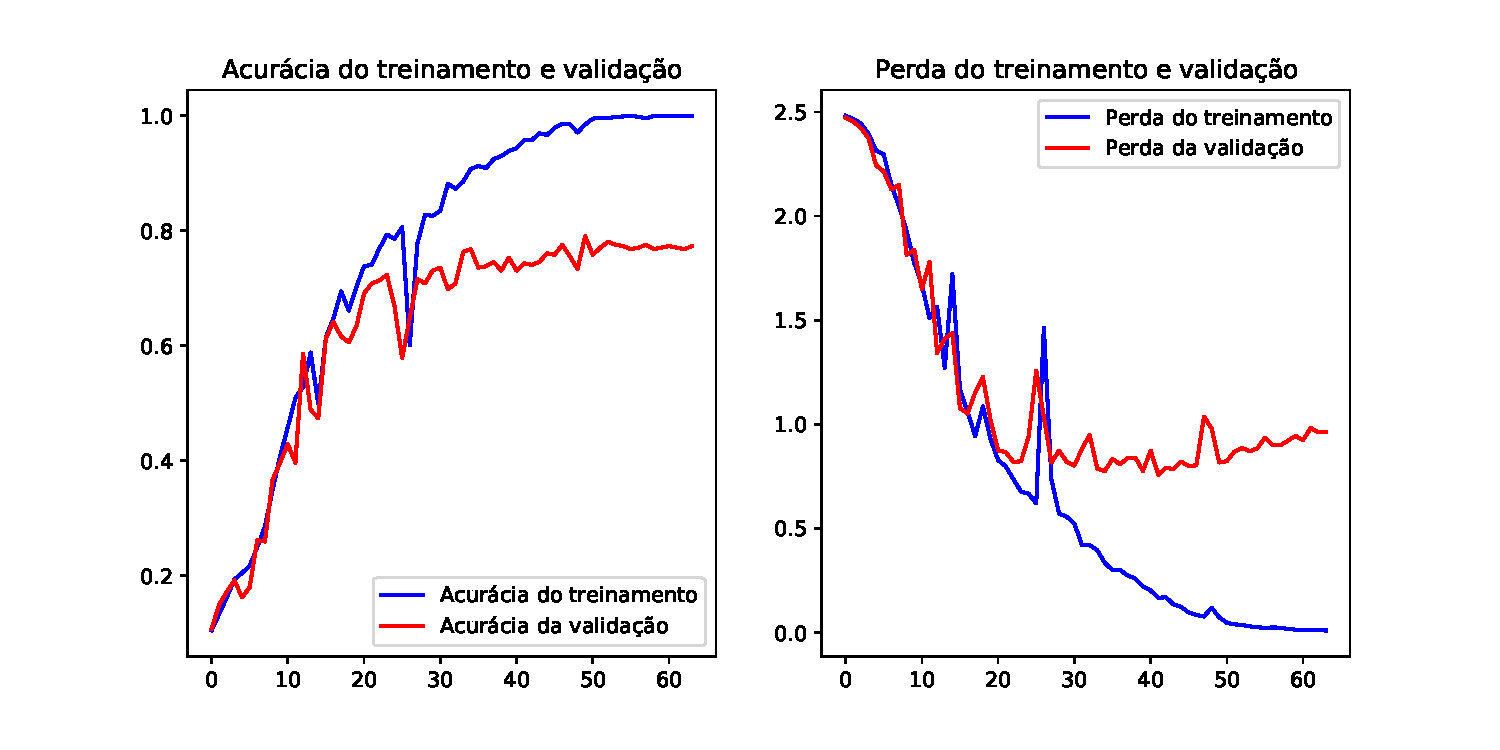
\includegraphics[width=1\textwidth]{images/history_lenet5.pdf}
\caption{\label{fig:grafico01}Acurácia e perda comparadas com treinamento e validação}
\end{figure}


\begin{figure}[!htb]
\centering
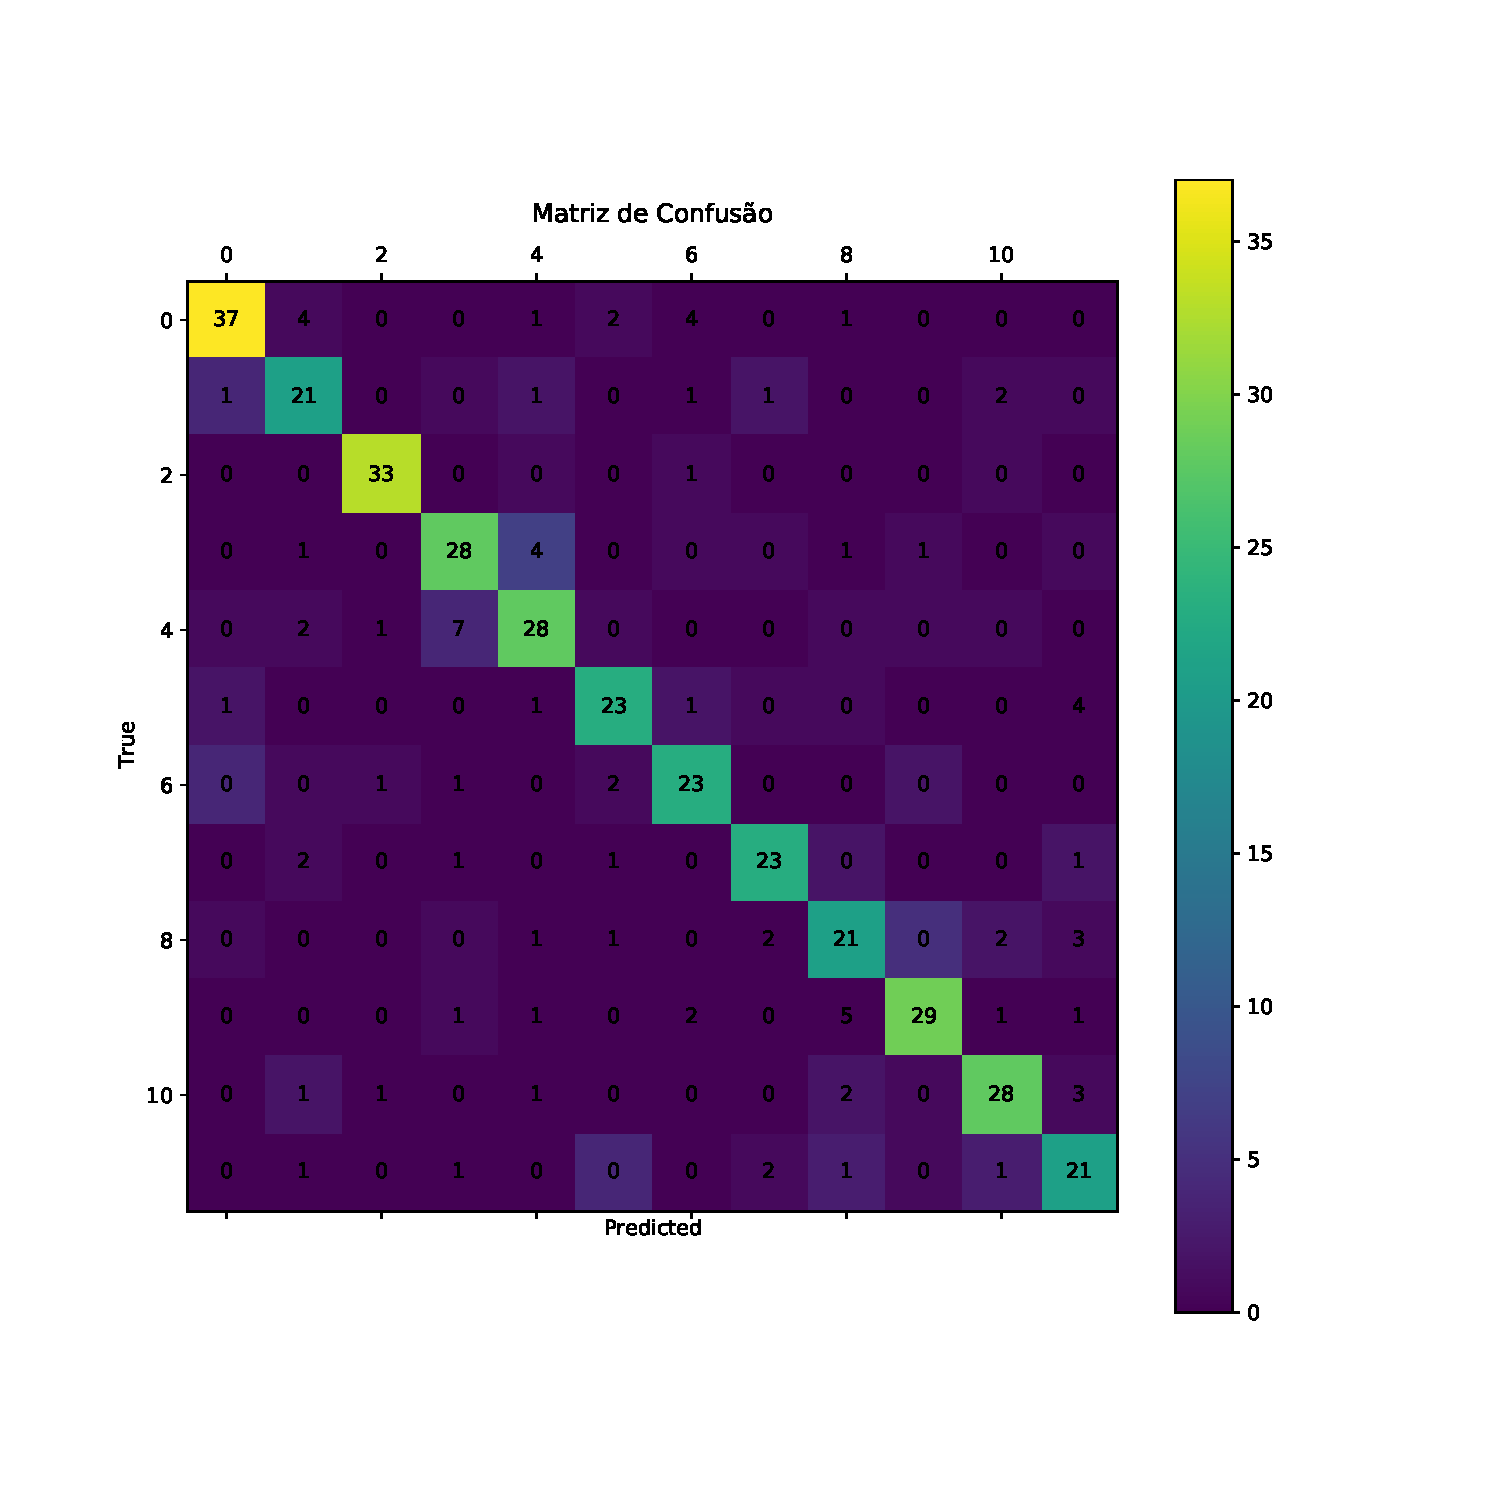
\includegraphics[width=0.7\textwidth]{images/cm_lenet5.pdf}
\caption{\label{fig:grafico01}Matrix de confusão}
\end{figure}

\clearpage

\subsection{Outra CNN}

Será apresentado uma tabela com os valores encontrados para alguns dos experimentos, incluindo a apresentação dos gráficos e matrix confusão para o melhor resultado. Os parâmetros a serem alterados são: batch\_size, epochs, image size e activation.

\begin{table}[!htb]
  \centering
  \begin{tabular}{|c|c|c|c|}
    \hline
    \textbf{Experimento} & \textbf{Loss} & \textbf{Acurácia} & \textbf{Tempo de Execução (s)} \\ \hline
    \begin{tabular}[c]{@{}l@{}}Outra CNN, batch\_size=32, \\ epochs=100, image=32x32, \\ activation=relu\end{tabular}    & 1.14          & 0.80              & 13.47                           \\ \hline
    \begin{tabular}[c]{@{}l@{}}Outra CNN, batch\_size=64, \\ epochs=100, image=32x32, \\ activation=relu\end{tabular}    & 1.38          & 0.76              & 11.74                           \\ \hline
    \begin{tabular}[c]{@{}l@{}}Outra CNN, batch\_size=16, \\ epochs=100, image=32x32, \\ activation=relu\end{tabular}    & 1.44          & 0.71              & 21.95                           \\ \hline
    \begin{tabular}[c]{@{}l@{}}Outra CNN, batch\_size=16, \\ epochs=160, image=32x32, \\ activation=relu\end{tabular}    & 0.98          & 0.82              & 34.69                           \\ \hline
    \begin{tabular}[c]{@{}l@{}}Outra CNN, batch\_size=16, \\ epochs=160, image=32x32, \\ activation=relu\end{tabular}    & 0.98          & 0.82              & 34.69                           \\ \hline
    \begin{tabular}[c]{@{}l@{}}Outra CNN, batch\_size=16, \\ epochs=160, image=50x50, \\ activation=relu\end{tabular}    & 2.33          & 0.09             & 80.93                          \\ \hline
    \begin{tabular}[c]{@{}l@{}}Outra CNN, batch\_size=128, \\ epochs=160, image=50x50, \\ activation=relu\end{tabular}    & 0.96          & 0.83             & 50.10                          \\ \hline
      \begin{tabular}[c]{@{}l@{}}Outra CNN, batch\_size=128, \\ epochs=160, image=48x48, \\ activation=relu\end{tabular}    & \textbf{0.55}          & \textbf{0.89}             & \textbf{31.37}                          \\ \hline
  \end{tabular}
  \caption{Resultados para outra CNN}
  \label{tab:experiment_simple_cnn_results}
\end{table}

\begin{figure}[!htb]
\centering
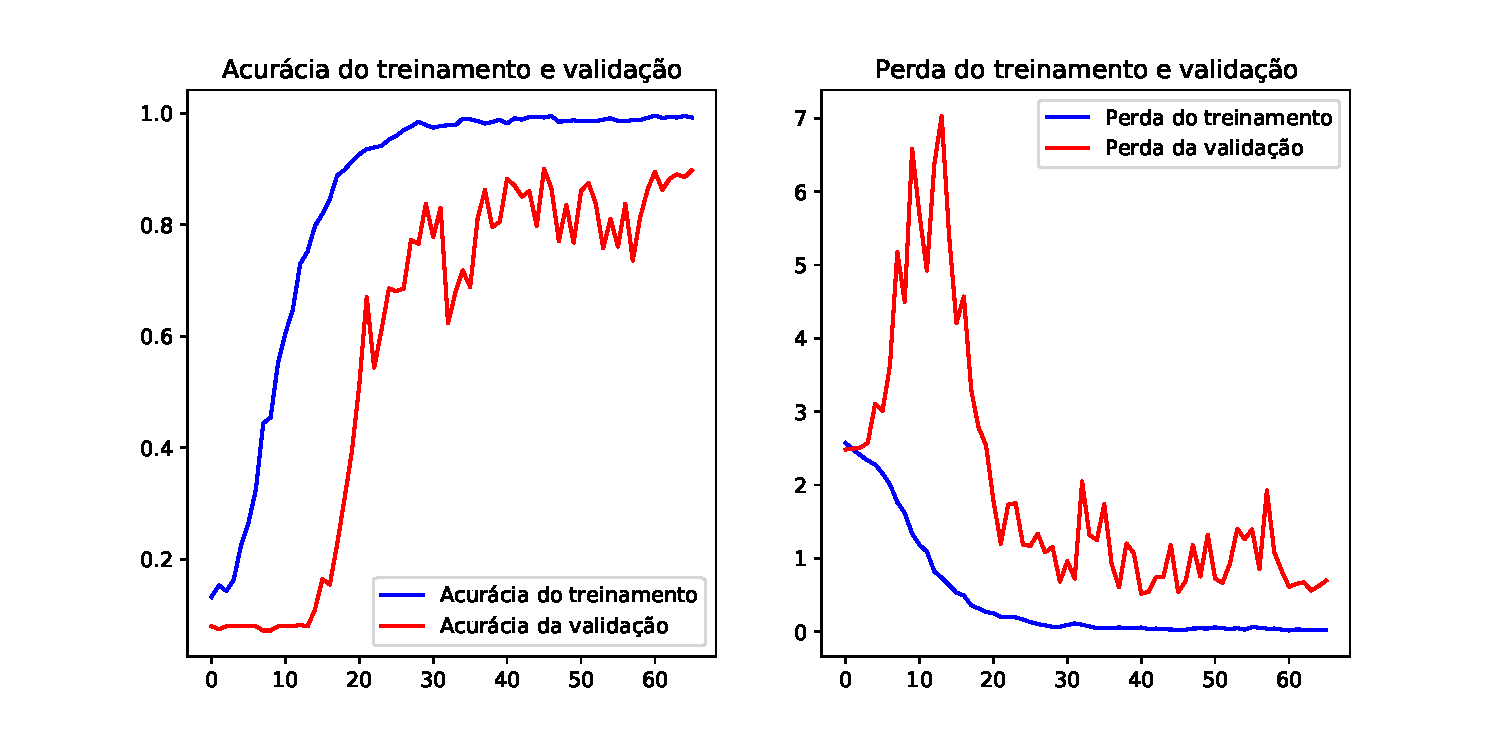
\includegraphics[width=1\textwidth]{images/history_simple_cnn.pdf}
\caption{\label{fig:grafico01}Acurácia e perda comparadas com treinamento e validação}
\end{figure}


\begin{figure}[!htb]
\centering
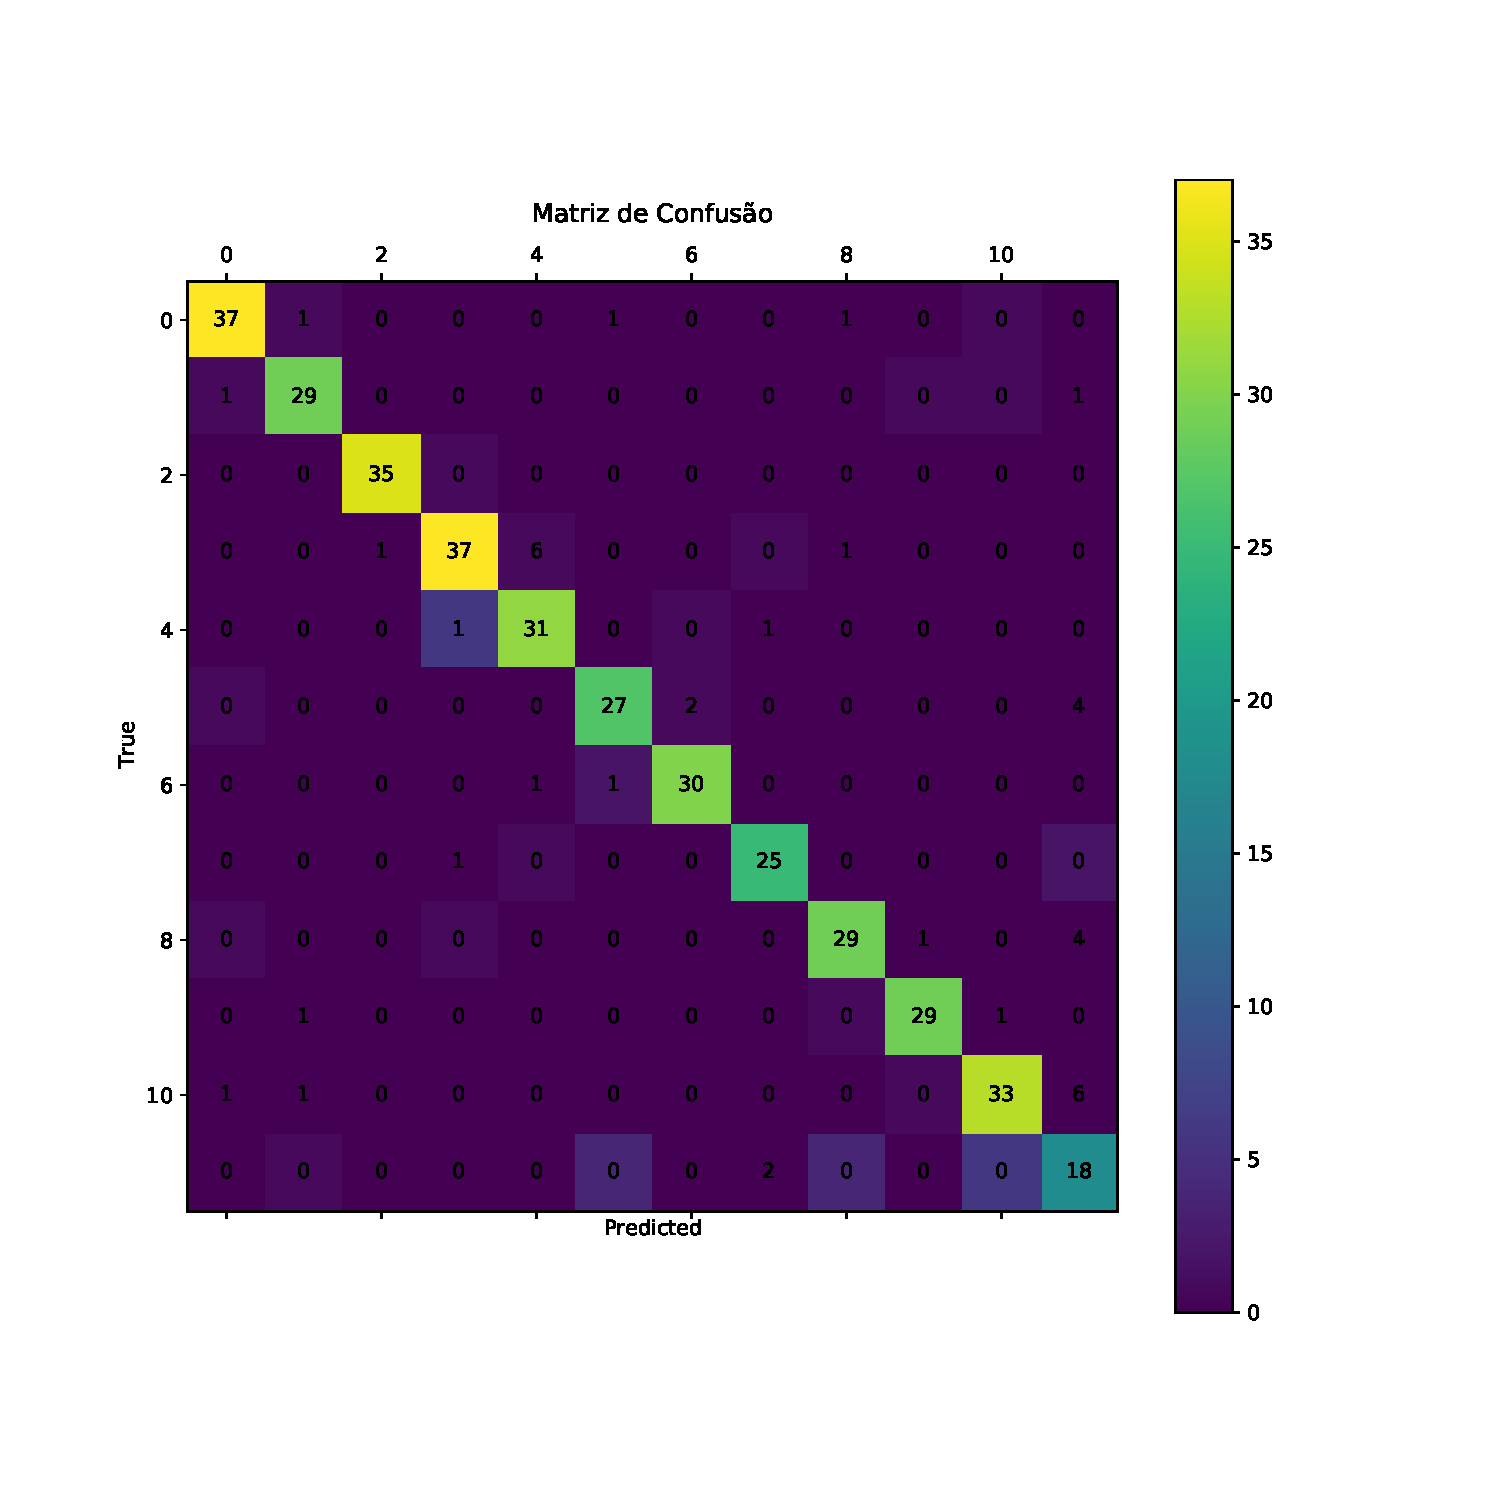
\includegraphics[width=0.7\textwidth]{images/cm_simple_cnn.pdf}
\caption{\label{fig:grafico01}Matrix de confusão}
\end{figure}

Esse CNN faz uso de um callback chamado EarlyStop, uma implementação do Keras que utiliza a piora na curva de loss como critério de parada. Apesar das épocas utilizadas serem grandes, a maioria das execuções terminam sem atingir o número limite de épocas.

\clearpage

\subsection{LeNet-5 com dados augumentados}

A mesma CNN LeNet-5, agora rodando com uma base maior de imagens, geradas pelo processo descrito na seção \ref{section:data_augmented}. A quantidade de imagens utilizadas no treinamento é de 37358. Os resultados podem ser vistos na tabela abaixo.

\begin{table}[!htb]
  \centering
  \begin{tabular}{|c|c|c|c|}
    \hline
    \textbf{Experimento} & \textbf{Loss} & \textbf{Acurácia} & \textbf{Tempo de Execução (s)} \\ \hline
      \begin{tabular}[c]{@{}l@{}}LeNet-5 aug, batch\_size=128, \\ epochs=64, image=50x50, \\ activation=relu\end{tabular}    & 2.02          & 0.82              & 319.85                           \\ \hline
        \begin{tabular}[c]{@{}l@{}}LeNet-5 aug, batch\_size=128, \\ epochs=13, image=50x50, \\ activation=relu\end{tabular}    & \textbf{0.47}          & \textbf{0.85}              & \textbf{74.565}                           \\ \hline
      \begin{tabular}[c]{@{}l@{}}LeNet-5 aug, batch\_size=32, \\ epochs=64, image=28x28, \\ activation=relu\end{tabular}    & 2.73          & 0.81              & 249.04                           \\ \hline
      \begin{tabular}[c]{@{}l@{}}LeNet-5 aug, batch\_size=128, \\ epochs=64, image=32x32, \\ activation=relu\end{tabular}    & 0.52          & 0.83              & 48.62                           \\ \hline
      \begin{tabular}[c]{@{}l@{}}LeNet-5 aug, batch\_size=64, \\ epochs=14, image=32x32, \\ activation=relu\end{tabular}    & 0.81          & 0.81              & 56.08                           \\ \hline
      \begin{tabular}[c]{@{}l@{}}LeNet-5 aug, batch\_size=32, \\ epochs=14, image=32x32, \\ activation=relu\end{tabular}    & 0.76          & 0.81              & 64.367                           \\ \hline
  \end{tabular}
  \caption{Resultados para LeNet-5}
  \label{tab:experiment_lenet5_noaug_32_reults}
\end{table}

Os gráficos de acurácia e perda com o melhor desempenho.

\begin{figure}[!htb]
\centering
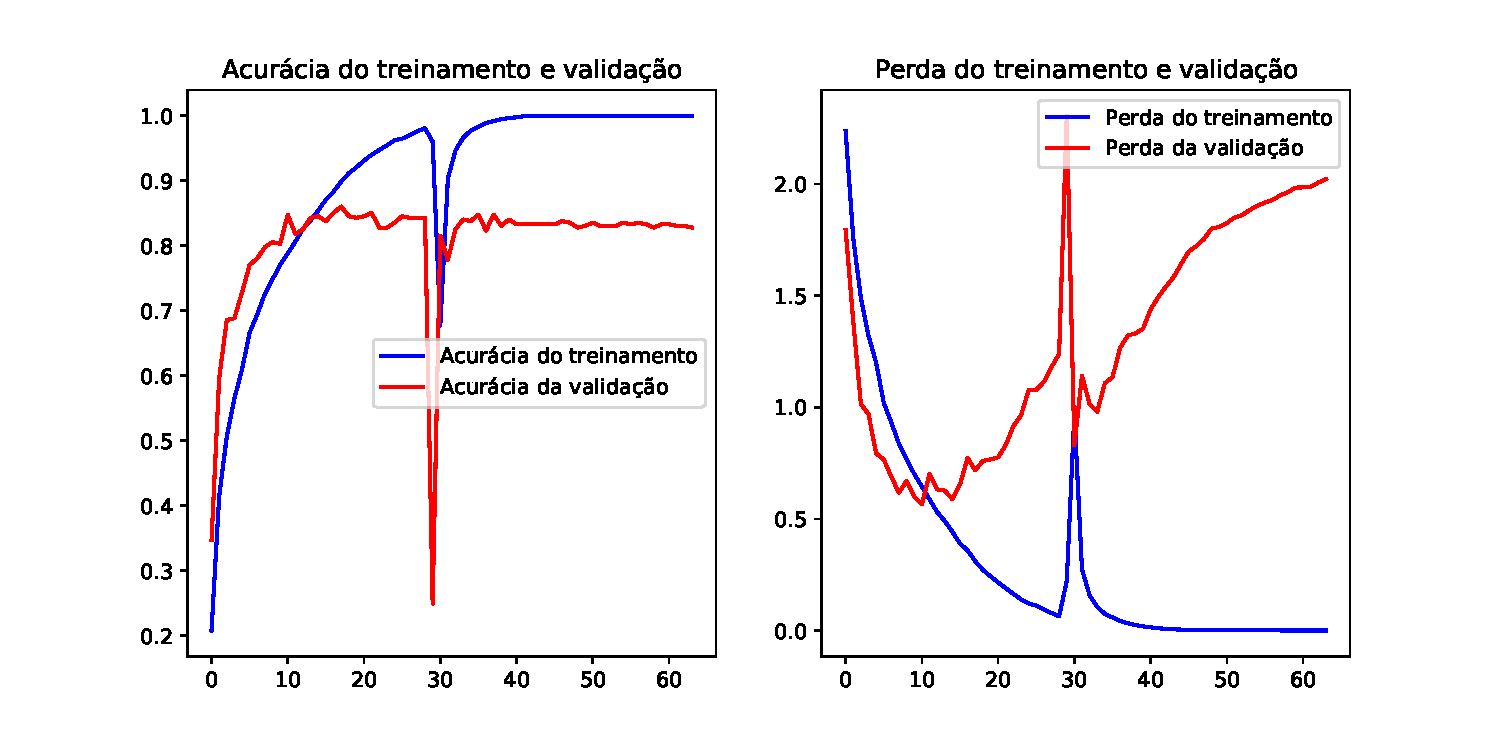
\includegraphics[width=1\textwidth]{images/history_lenet5_augmented.pdf}
\caption{\label{fig:grafico01}Acurácia e perda comparadas com treinamento e validação}
\end{figure}

O gráfico da matriz de confusão com o melhor desempenho.

\begin{figure}[!htb]
\centering
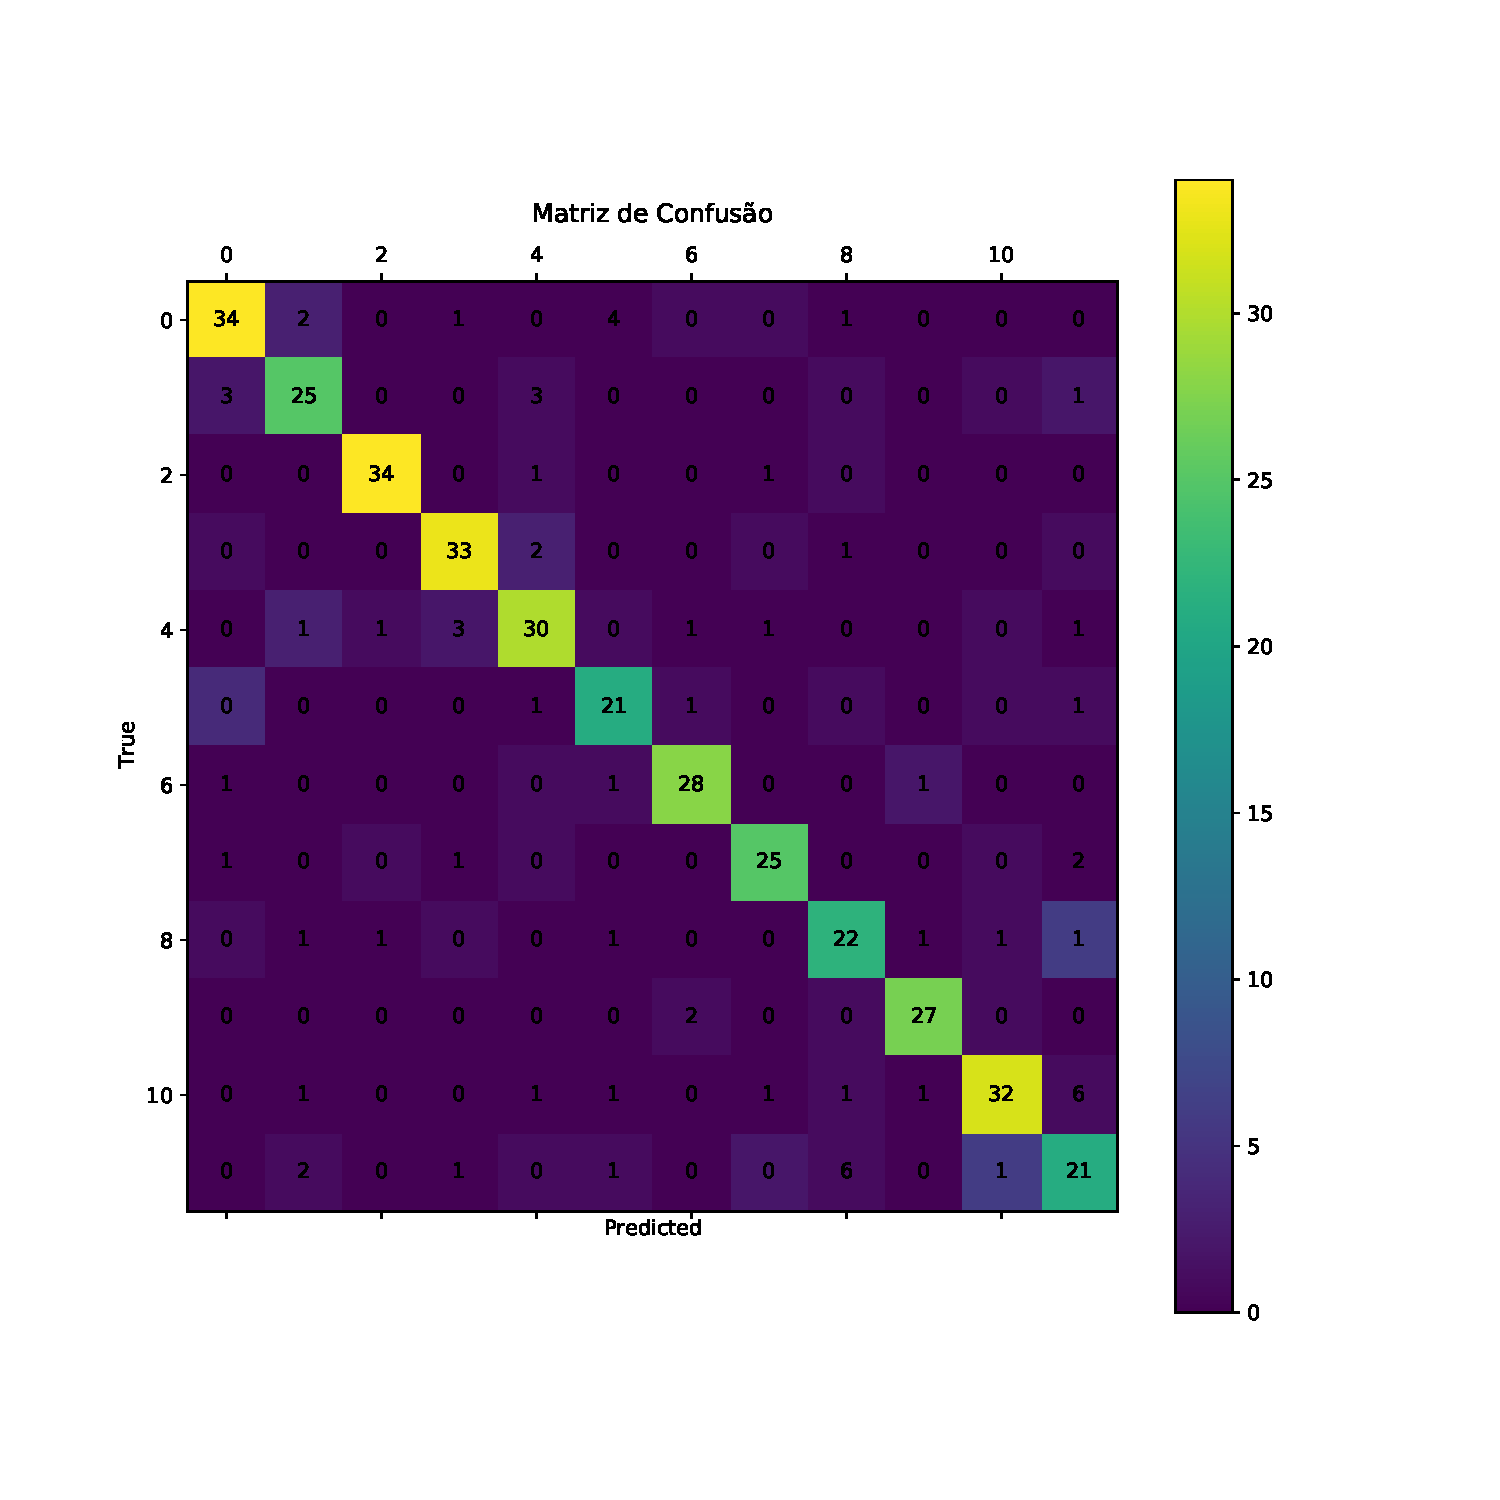
\includegraphics[width=0.7\textwidth]{images/cm_lenet5_augmented.pdf}
\caption{\label{fig:grafico01}Matrix de confusão}
\end{figure}


\clearpage

\subsection{Outra CNN com dados augumentados}

Utilizando uma base de imagens com 37358 imagens, sendo 36000 imagens novas, geradas pelo processo descrito na seção \ref{section:data_augmented}.  

\begin{table}[!htb]
  \centering
  \begin{tabular}{|c|c|c|c|}
    \hline
    \textbf{Experimento} & \textbf{Loss} & \textbf{Acurácia} & \textbf{Tempo de Execução (s)} \\ \hline
    \begin{tabular}[c]{@{}l@{}}Outra CNN augumentada, \\ batch\_size=128, epochs=160, \\ image=48x48\end{tabular}    & \textbf{0.53}          & \textbf{0.91}              & \textbf{449.74}                           \\ \hline
    \begin{tabular}[c]{@{}l@{}}Ooutra cnn augumentada, \\ batch\_size=32, epochs=100, \\ image=32x32\end{tabular}    & 1.30          & 0.72              & 231.25                           \\ \hline
    \begin{tabular}[c]{@{}l@{}}Outra cnn augumentada, \\ batch\_size=64, epochs=160, \\ image=48x48\end{tabular}    & 0.60          & 0.89              & 465.77                           \\ \hline
  \end{tabular}
  \caption{Resultados para outra CNN}
  \label{tab:experiment_simple_cnn_results}
\end{table}

\begin{figure}[!htb]
\centering
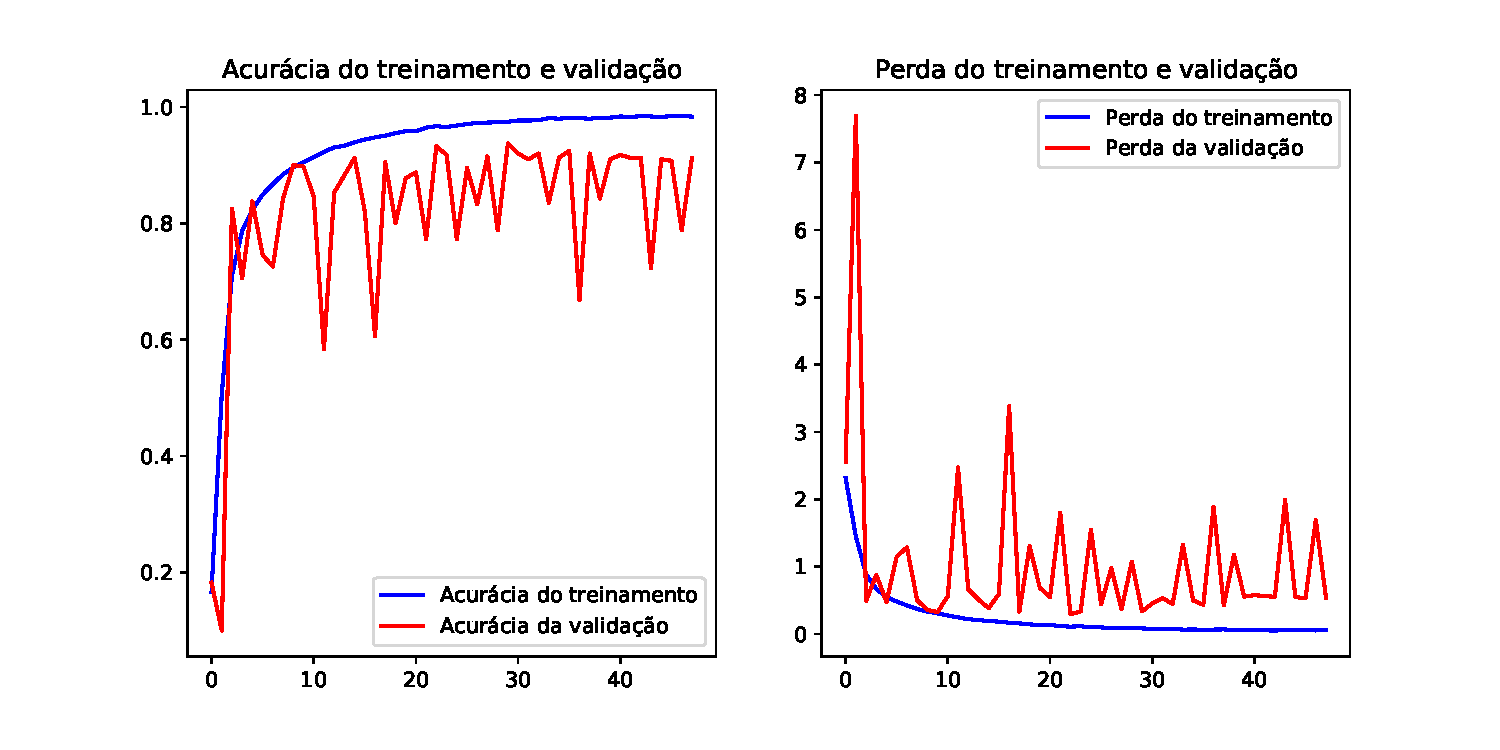
\includegraphics[width=1\textwidth]{images/history_simple_cnn_augmented.pdf}
\caption{\label{fig:grafico01}Acurácia e perda comparadas com treinamento e validação}
\end{figure}


\begin{figure}[!htb]
\centering
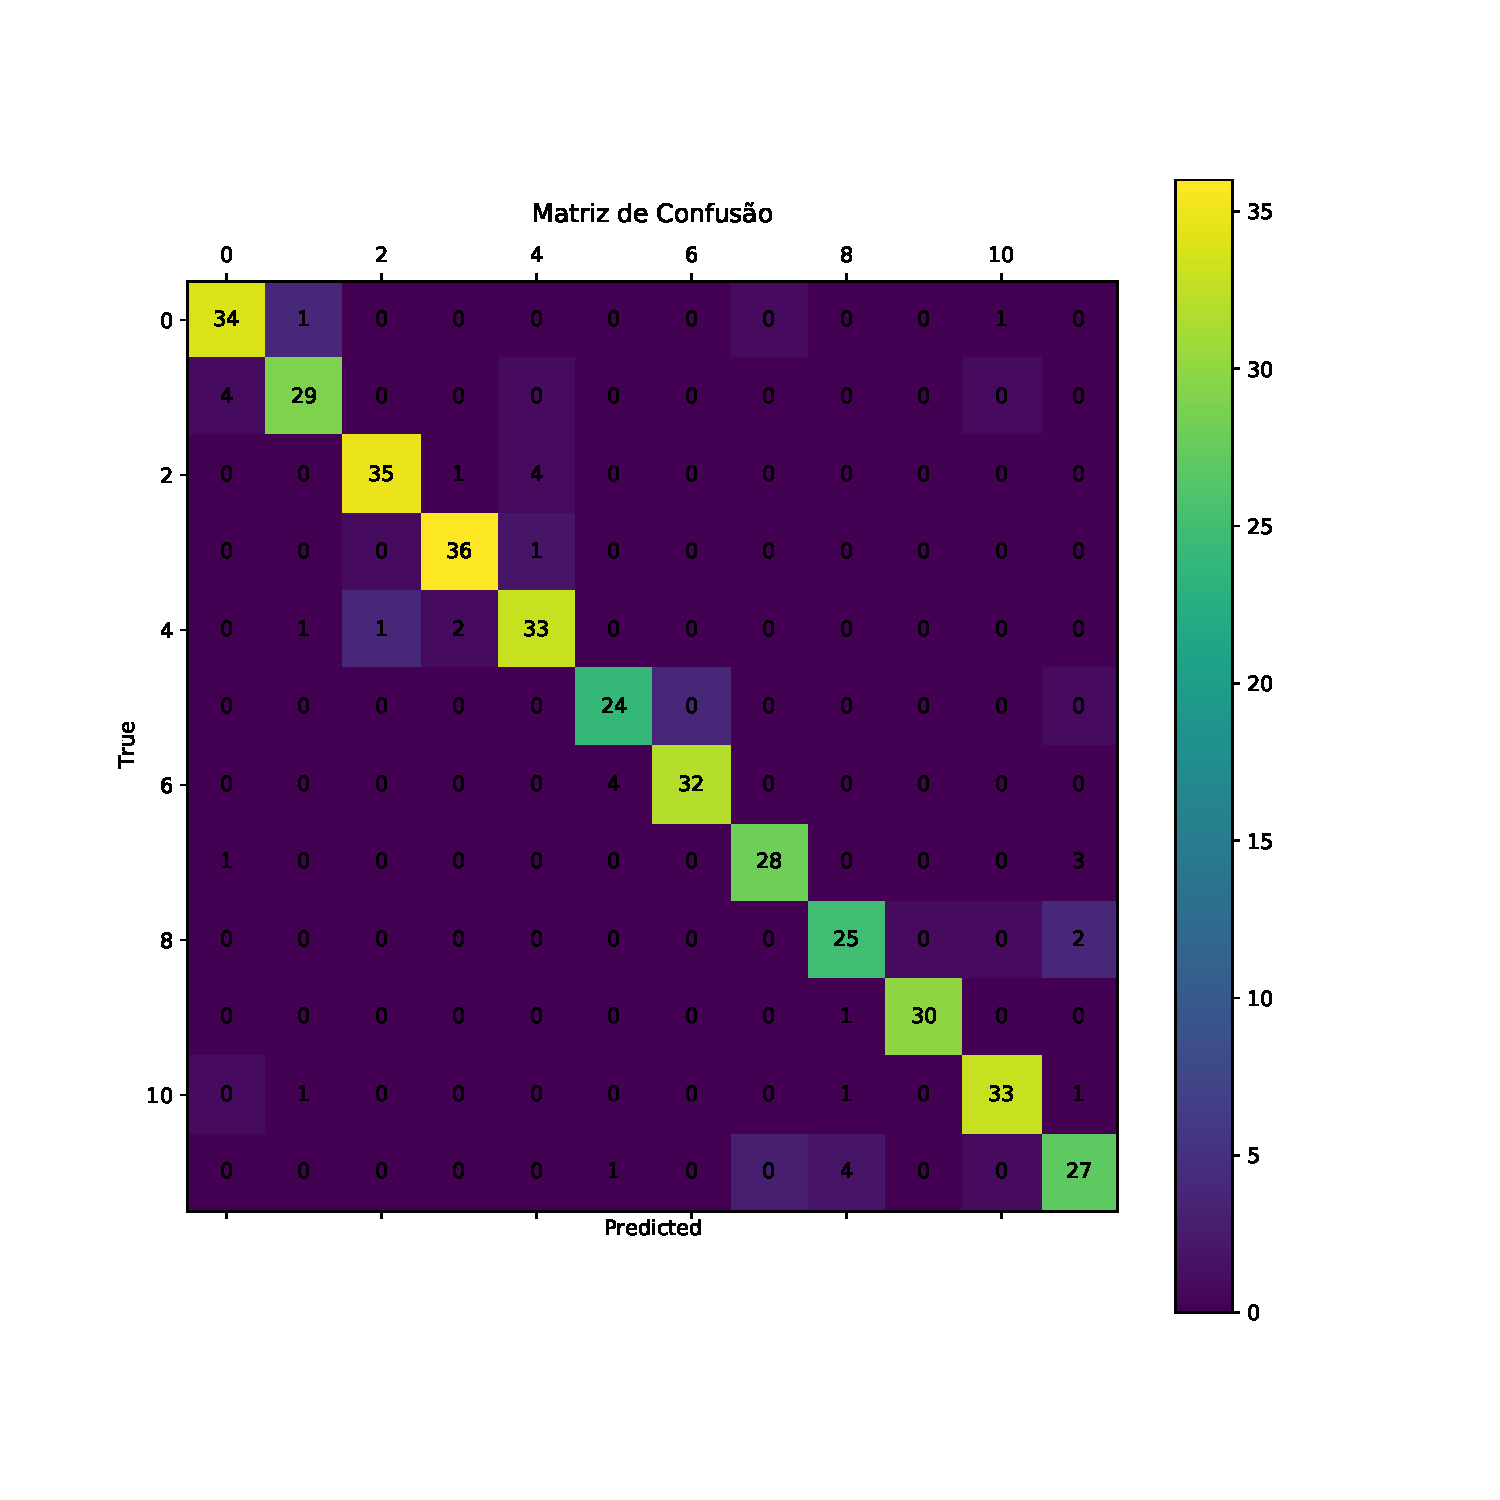
\includegraphics[width=0.7\textwidth]{images/cm_simple_cnn_augmented.pdf}
\caption{\label{fig:grafico01}Matrix de confusão}
\end{figure}

\clearpage

\section{Conclusão dos experimentos}

A primeira conclusão é que os dados de treino não são suficientes para aumentar a acurácia da validação.

Os parâmetros que mais afetaram o desempenho das CNNs foram o tamanho do lote, batch\_size, e o tamanho da imagem. Inicialmente a LeNet-5 contava com tamanho 28x28, mas normalmente ela é utilizada com tamanho 32x32, nos testes realizados o desempenho aumentou quando o recorte chegou ao tamanho 50x50.

No caso da outra CNN, o melhor recorte de imagem encontrado foi 48x48, com lotes de 128 para treinamento da rede. Como lotes grandes tem a tendência de overfitting, a estratégia estava em diminuir o tamanho das épocas.

Um problema comum ao modelo sendo treinado, é que dado o número longo de épocas, o modelo pode entrar em overfitting o que por sua vez aumenta a métrica loss da validação.

Com os dados gerados através da técnica de augumentação os modelos conseguiram aumentar sua acurácia, tanto para LeNet-5, quanto a Outra CNN.

Acredito que dois filtros poderiam melhorar os resultados. Um deles que pudesse deixar a imagem mais clara ou escura, e outro filtro que pudesse incluir ruídos diretamente nas linhas, apagando partes do traço, para tentar reproduzir uma caneta falhando ou os saltos da escrita das letras que podem variar de pessoa para pessoa.

O parâmetro que se mostrou mais prejudicial a sua alteração foi a função de ativação. Por isso os testes seguem a estratégia da rede original. Alguns testes mostraram que o simples fato de alterar a função de ativação nas camadas de aprendizado, causava um impacto tão negativo que muitas vezes o modelo não conseguia sair de 10\% de acurácia.

\section{Duas redes pré-treinadas na ImageNet}

\subsection{CNN Inception-v4}

Para esse experimento, utilizou-se a CNN Inception v4 com os pesos de uma rede pré-treinada.

Para garantir que as camadas não sejam treinadas, mantendo assim os pesos originais foi utilizado o código:

\begin{lstlisting}[caption={CNN escolhida},captionpos=b,frame=single,label={code:modelo_personalizado}, language=Python]
for l in model.layers: 
    if l is not None: l.trainable = False
\end{lstlisting}

O melhor resultado com as 1578 imagens originais.

\begin{table}[!htb]
  \centering
  \begin{tabular}{|c|c|c|c|}
    \hline
    \textbf{Experimento} & \textbf{Loss} & \textbf{Acurácia} & \textbf{Tempo de Execução (s)} \\ \hline
    \begin{tabular}[c]{@{}l@{}}Inception-v4, \\ batch\_size=128, epochs=160, \\ image=48x48\end{tabular}    & \textbf{0.82}          & \textbf{0.07}              & \textbf{17.69}                           \\ \hline
  \end{tabular}
  \caption{Resultados para Inception-v4}
  \label{tab:experiment_simple_cnn_results}
\end{table}

\begin{figure}[!htb]
\centering
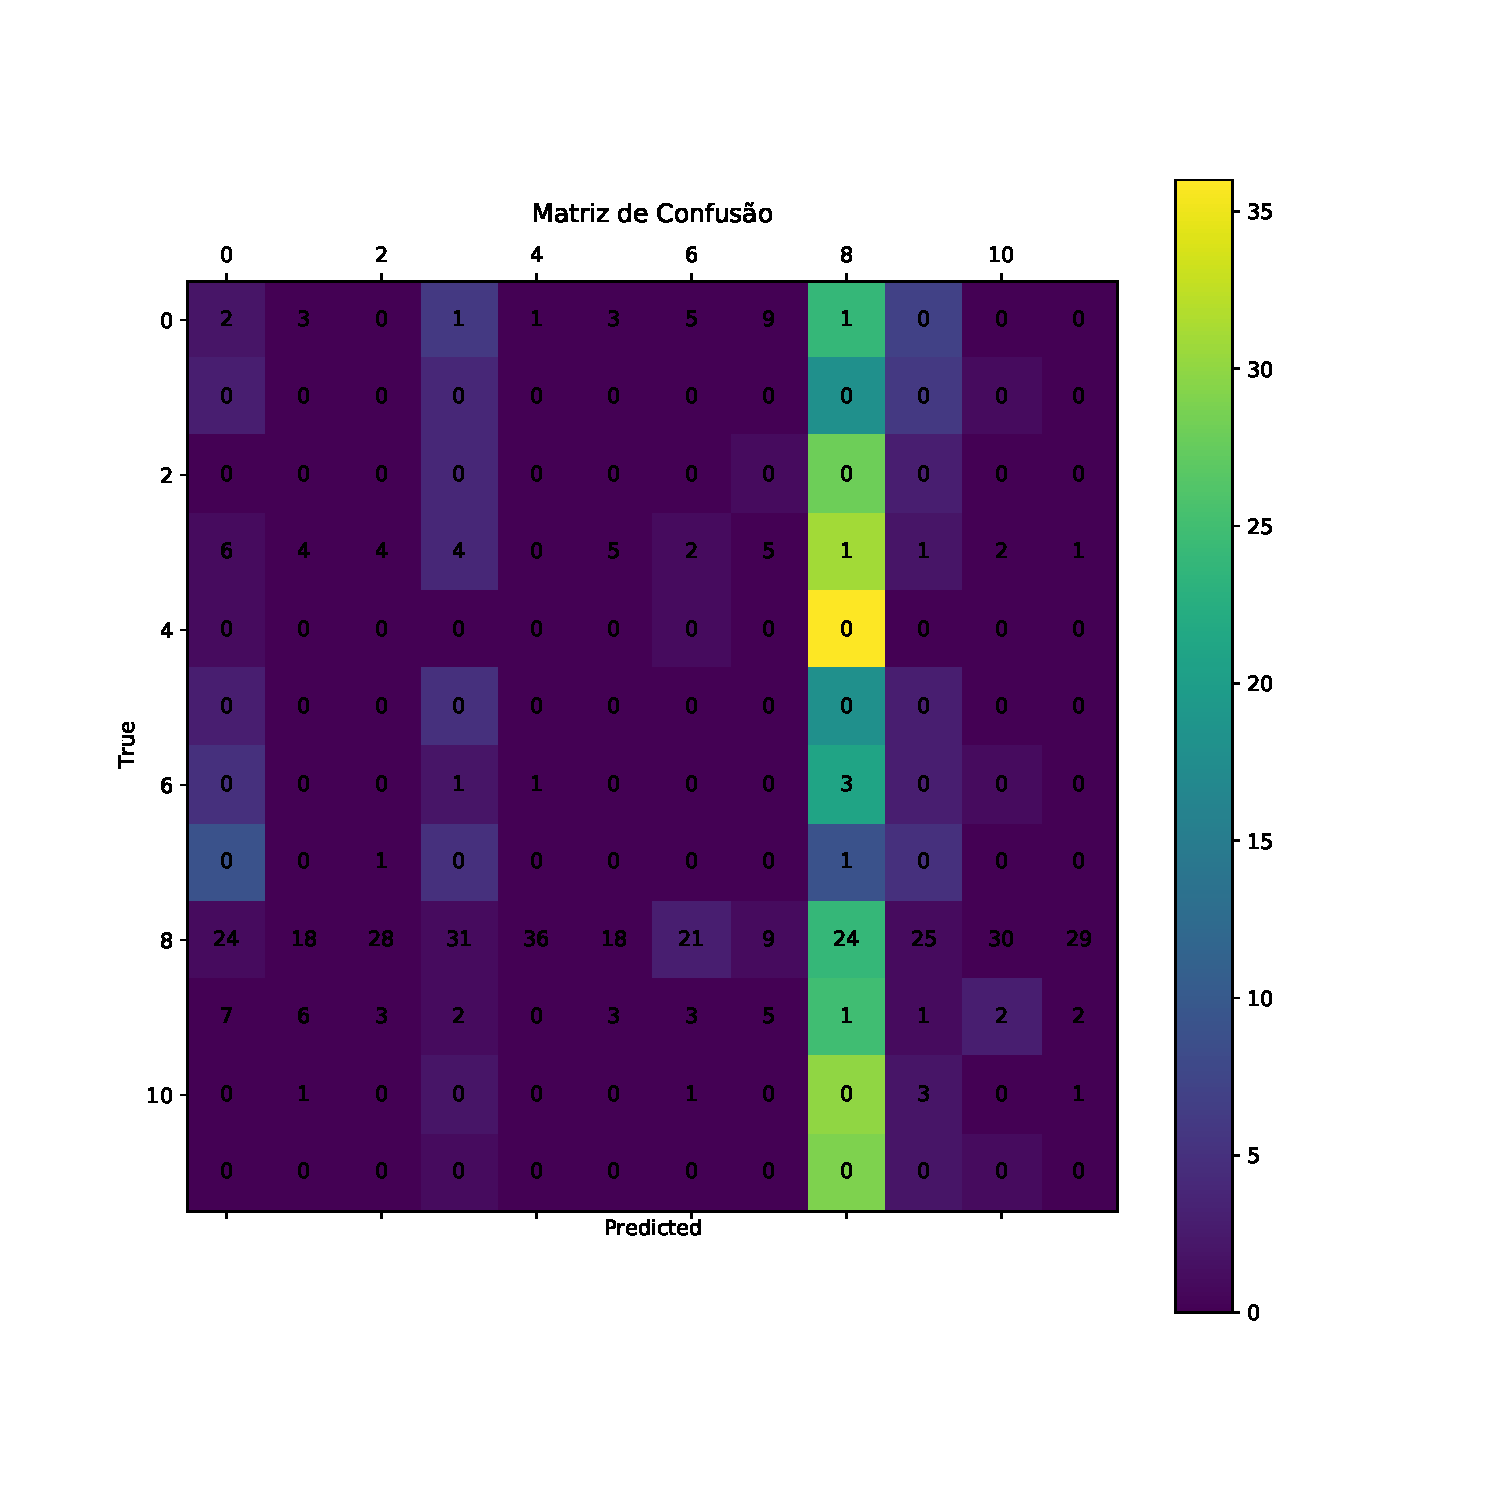
\includegraphics[width=0.7\textwidth]{images/cm_inception_v4.pdf}
\caption{\label{fig:grafico01}Matrix de confusão}
\end{figure}

\subsection{CNN VGG16}

Para esse experimento, utilizou-se a CNN VGG16 da ImageNet com os pesos de uma rede pré-treinada ``imagenet''.

A CNN VGG16 carregada direto da biblioteca é um modelo funcional, portanto é necessário modificar sua entrada e sua saída para aceitar parâmetros diferentes. Por isso, um novo método para carregar a CNN foi criado, já que a original tem 1000 classes e estamos utilizando para 12 classes. Mesmo sem essa modificação, é possível fazer o predict das classes, mas ficará esparsa em uma matriz de 1000, tornando o método para gerar a matriz de confusão incompatível, já que os labels tem 12 níveis apenas.

\begin{lstlisting}[caption={CNN escolhida},captionpos=b,frame=single,label={code:modelo_personalizado}, language=Python]

def vgg16(img_rows, img_cols, num_classes):
  #Get back the convolutional part of a VGG network trained on ImageNet
  model_vgg16_conv = VGG16(weights='imagenet', include_top=False, input_shape=(img_rows, img_cols, 3), classes=num_classes)
    
  #Create your own input format
  input = Input(shape=(img_rows, img_cols, 3), name = 'image_input')

  #Use the generated model 
  output_vgg16_conv = model_vgg16_conv(input)

  #Add the fully-connected layers 
  x = Flatten(name='flatten')(output_vgg16_conv)  
  x = Dense(num_classes, activation='softmax', name='predictions')(x)

  #Create your own model 
  model = Model(inputs=input, outputs=x)

  #In the summary, weights and layers from VGG part will be hidden, but they will be fit during the training
  # my_model.summary()

  # Say not to train first layer (ResNet) model. It is already trained
  for l in model.layers:
    if l is not None: l.trainable = False
  return model
\end{lstlisting}

A matriz de confusão para o experimento utilizando os valores padrões.

\begin{table}[!htb]
  \centering
  \begin{tabular}{|c|c|c|c|}
    \hline
    \textbf{Experimento} & \textbf{Loss} & \textbf{Acurácia} & \textbf{Tempo de Execução (s)} \\ \hline
    \begin{tabular}[c]{@{}l@{}}VGG16, \\ batch\_size=32, epochs=64, \\ image=224x224\end{tabular}    & \textbf{2.69}          & \textbf{0.11}              & \textbf{6.56}                           \\ \hline
  \end{tabular}
  \caption{Resultados para VGG16}
  \label{tab:experiment_simple_cnn_results}
\end{table}

\begin{figure}[!htb]
\centering
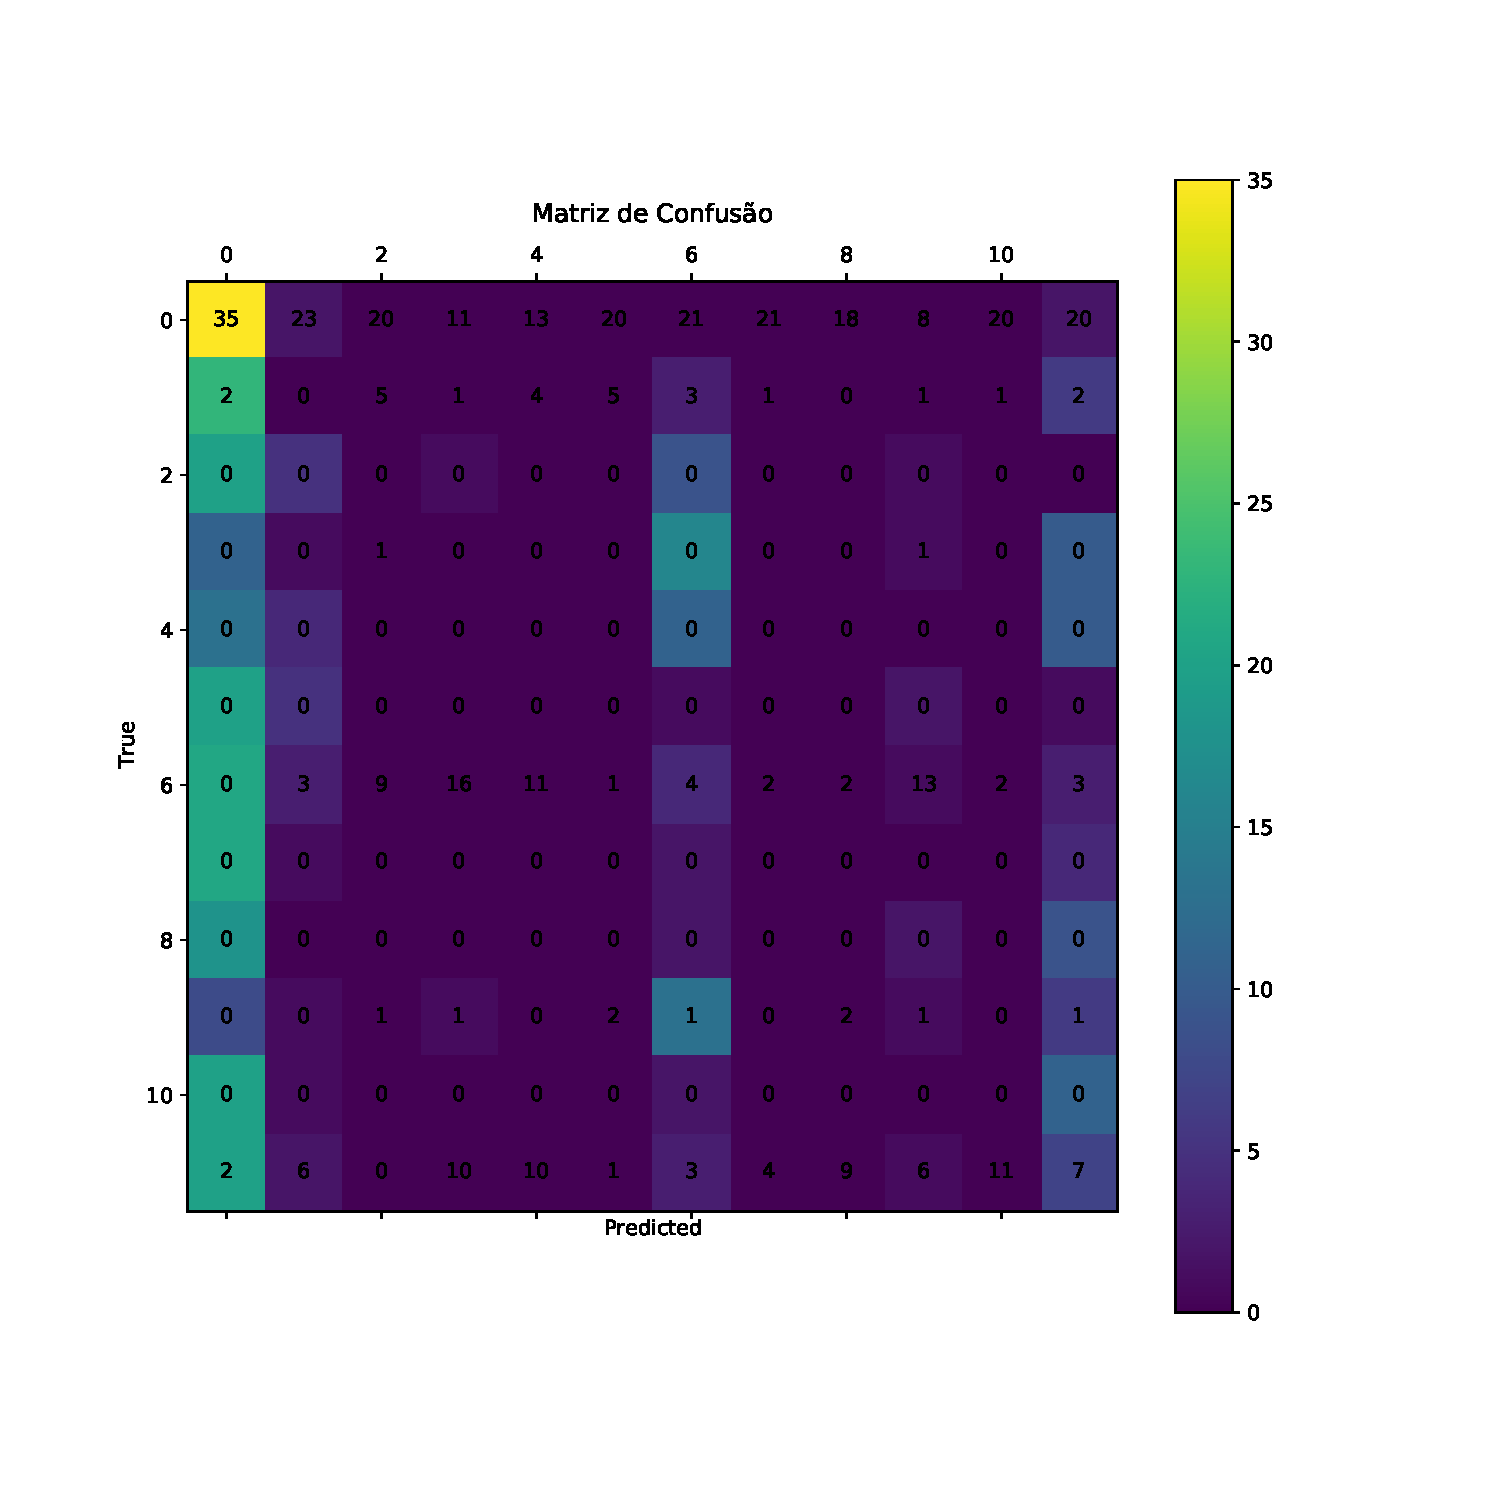
\includegraphics[width=0.7\textwidth]{images/cm_vgg16.pdf}
\caption{\label{fig:grafico01}Matrix de confusão}
\end{figure}

\section{Conclusão sobre as duas redes pré-treinadas da ImageNet}

Como as duas redes foram treinadas para classificar 1000 itens, sua rede está calibrada para um propósito diferente daquela que estamos estudando. Mesmo assim, como explicado em sala de aula, a mesma pode ser utilizada para \textit{feature extraction}.

Realizando os testes como instruído ocorreu um problema para trabalhar com a base augmentada, para o tamanho padrão das redes, a Inception v4, trabalha com imagens de 299 e VGG16 com 224. O que acontece é que as imagens são carregadas em memória, para um número grande de testes a memória do Colab não é suficiente para rodar os testes com dados augumentados. Outra estratégia para lidar com o problema deve ser implementada. Uma possível solução seria utilizar o método generator do Keras, que faz a carga das imagens por Batch. Verificando a estrutura do train.txt e as mudanças necessárias para criar um sistema de arquivo compatível, chegou-se a conclusão que seria preciso criar uma nova ferramenta. Devido ao grande número de atividades para criar os testes já necessários, o mesmo não foi criado. Portanto, apenas testes sem dados augumentados foram apresentados. Sem os testes, mas já reparando no resultado ruim das redes pré-treinadas, supõe-se que o resultado não seja muito diferente.

\section{Extração de características - \textit{Feature Extraction}}

Para realizar a extração de caracteristicas faremos uso da CNN Inception v4. Mas para isso é necessário alterar o número de características de 12 para 1000, valor original para a ImageNet. O script utilizado pode ser visto na listagem abaixo.

\begin{lstlisting}[caption={CNN escolhida},captionpos=b,frame=single,label={code:modelo_personalizado}, language=Python]
## Star Time
checkpoint_time = get_time()

INPUT_FILE_TEST = "./ml_lab3/test.txt"
OUTPUT_FILE_TEST = "./ml_lab3/svm/test.svm"
INPUT_FILE_TRAIN = TRAIN_FINAL
OUTPUT_FILE_TRAIN = "./ml_lab3/svm/train.svm"
IMG_ROWS = 100
IMG_COLS = 100
DIR_DATASET = "./ml_lab3/"

model = get_model()

# Train
extract_features(model, INPUT_FILE_TRAIN, OUTPUT_FILE_TRAIN, IMG_ROWS, IMG_COLS, DIR_DATASET)

# Test
extract_features(model, INPUT_FILE_TEST, OUTPUT_FILE_TEST, IMG_ROWS, IMG_COLS, DIR_DATASET)

## Execution Time
print(f'Execution Time: {get_time_diff(checkpoint_time)}')

print('DONE')
\end{lstlisting}

O arquivo de treino possui as imagens augumentadas e o tamanho da imagem foi alterada para 100x100, para evitar problemas de memória.

O processo tomou aproximamente 67 segundos para cada lote de 1000 arquivos, resultando no total de 45 minutos para extrair as características de 37759 imagens. O arquivo final é um arquivo train.svm, qu possui um tamanho aproximado de 608MB.

Devido ao tamanho dos arquivos e a execução estar acontecendo em ambiente virtualizado, no Colab, decidiu-se apenas um lote de testes com a CNN Inception v4.

\section{Classificador SVM}

Nesta etapa utiliza-se o classificador SVM para realizar a classificação das imagens.

Para fazer as escolhas das melhores características utilizou-se o script abaixo. Neste script é utilizado o GridSearchCV da biblioteca do scikit learn, para executar uma validação cruzada dos parâmetros \textbf{C}, e \textbf{gamma}. Dois kernels são testados, o linear e o radial. O resultado é o melhor modelo testado contra a base de dados.

\begin{lstlisting}[caption={CNN escolhida},captionpos=b,frame=single,label={code:modelo_personalizado}, language=Python]
## Star Time
checkpoint_time = get_time()

INPUT_TRAIN = "../ml_lab3/svm/train.svm"
INPUT_TEST = "../ml_lab3/svm/test.svm"

x_train, y_train = load_svmlight_file(INPUT_TRAIN)
x_test, y_test = load_svmlight_file(INPUT_TEST)

x_train = x_train.toarray()
x_test = x_test.toarray()

# Create the parameter grid based on the results of random search 
params_grid = [{'kernel': ['rbf'], 'gamma': [1e-3, 1e-4],
                     'C': [1, 10, 100, 1000]},
                    {'kernel': ['linear'], 'C': [1, 10, 100, 1000]}]

# Performing CV to tune parameters for best SVM fit 
svm_model = GridSearchCV(SVC(), params_grid, cv=5, verbose=1, n_jobs=-1)
svm_model.fit(x_train, y_train)
## Execution Time
print(f'Execution Time: {get_time_diff(checkpoint_time)}')
\end{lstlisting}

Os melhores parâmetros encontrados foram C = 1000, gamma = 0.001. A tabela abaixo apresenta os resultados de acurácia do melhor modelo.

\begin{table}[!htb]
  \centering
  \begin{tabular}{|c|c|c|c|}
    \hline
    \textbf{Experimento} & \textbf{F1 Score} & \textbf{Acurácia} & \textbf{Tempo de Execução (s)} \\ \hline
    \begin{tabular}[c]{@{}l@{}}SVM kernel rbf \\ C = 1000 \\ gamma = 1e-3\end{tabular}    & \textbf{0}          & \textbf{0.097}              & \textbf{0.177}                           \\ \hline
  \end{tabular}
  \caption{Resultado para o SVM}
  \label{tab:experiment_simple_cnn_results}
\end{table}

O resultado da matriz de confusão, a seguir, mostra que todos os valores ficaram na classe 0. Isso indica que o modelo está errado, provavelmente relacionado ao número de dimensões utilizados para classificação. Mesmo com esse resultado, o tempo para avaliação é de aproximadamente 74 minutos.

\begin{figure}[!htb]
\centering
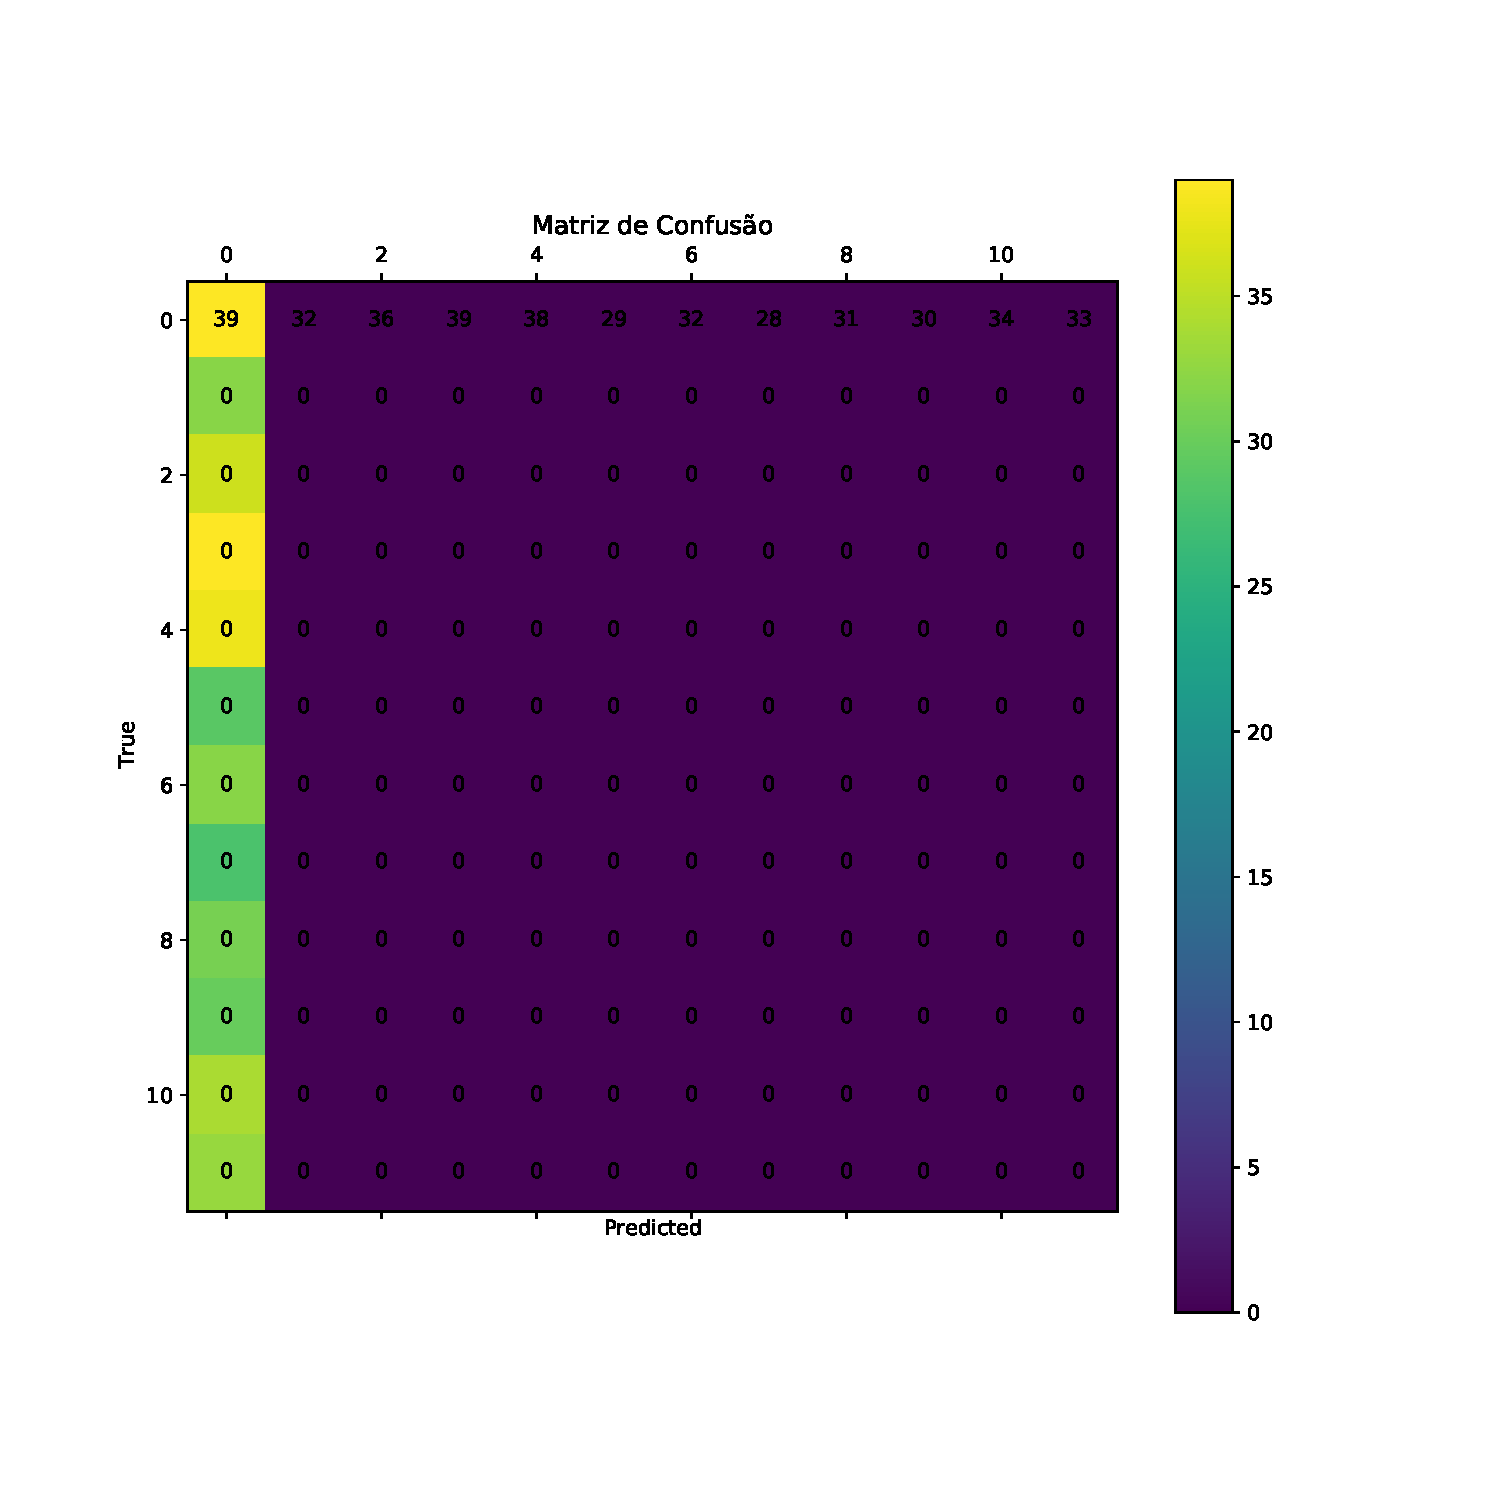
\includegraphics[width=0.7\textwidth]{images/cm_svm_rbf.pdf}
\caption{\label{fig:cm_svm_rfb}Matriz de confusão}
\end{figure}

\clearpage

\section{Referências}

\bibliographystyle{abntex2-num}
\bibliography{aaabib}

\end{document}

%% Exemplo de figura, copie e cole, substituindo os conteúdos.
\begin{figure}[H]
\centering
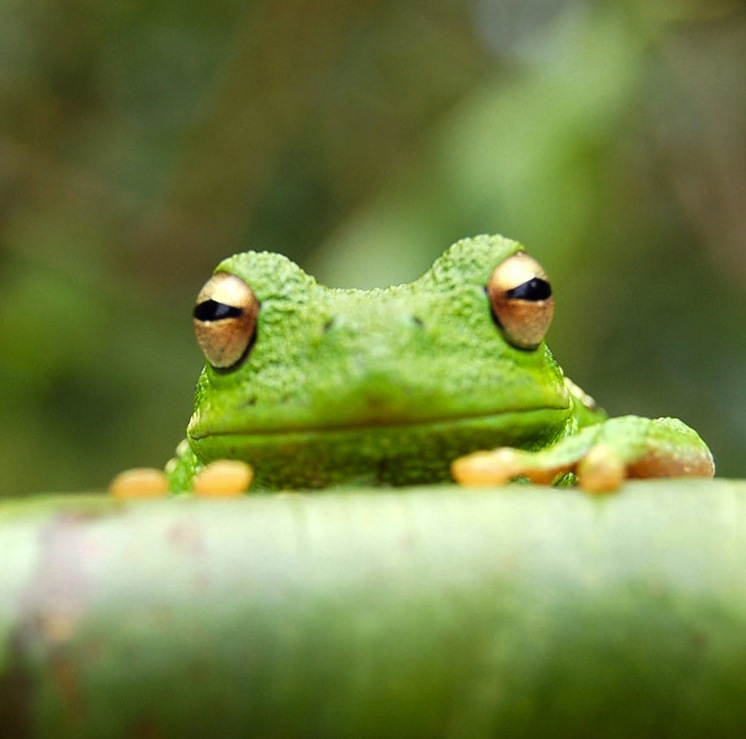
\includegraphics[width=0.3\textwidth]{frog.jpg}
\caption{\label{fig:frog}This frog was uploaded via the project menu.}
\end{figure}

%% Exemplo de tabela, copie e cole, substituindo os conteúdos.
\begin{table}[H]
\centering
\begin{tabular}{l|r}
Item & Quantity \\\hline
Widgets & 42 \\
Gadgets & 13
\end{tabular}
\caption{\label{tab:widgets}An example table.}
\end{table}

\begin{lstlisting}[caption={Relatório do algoritmo kNN},label={relatorio},language=Python]
features_extraction((20,69))
knn("features.txt", 3)
[[ 96   0   0   0   0   1   0   0   0   0]
 [  0  95   0   0   0   0   0   0   0   0]
 [  0   3 103   0   1   0   1   2   1   0]
 [  1   1   0  98   0   1   0   1   1   0]
 [  0   9   2   0  82   0   0   0   0   2]
 [  1   0   0   4   0  91   1   0   0   0]
 [  1   5   0   0   0   0 100   0   0   0]
 [  0   9   0   0   0   0   0  86   0   2]
 [  1   3   0   2   1   1   0   0  79   0]
 [  0   1   0   0   3   0   0   9   1  98]]
              precision    recall  f1-score   support

           0       0.96      0.99      0.97        97
           1       0.75      1.00      0.86        95
           2       0.98      0.93      0.95       111
           3       0.94      0.95      0.95       103
           4       0.94      0.86      0.90        95
           5       0.97      0.94      0.95        97
           6       0.98      0.94      0.96       106
           7       0.88      0.89      0.88        97
           8       0.96      0.91      0.93        87
           9       0.96      0.88      0.92       112

    accuracy                           0.93      1000
   macro avg       0.93      0.93      0.93      1000
weighted avg       0.93      0.93      0.93      1000

0.928
\end{lstlisting}

\section{Atividade - II}

\textbf{Atividade:} Indique qual é o classificador que tem o melhor desempenho com poucos dados = 1000 exemplos. A tabela \ref{tab:tamanho1000} apresenta os resultados a serem analisados.

\begin{table}[H]
\centering
\begin{tabular}{|l|l|l|}
\hline
Classificador & \begin{tabular}[c]{@{}l@{}}Tamanho do \\ bloco de treino\end{tabular} & Acurácia \\ \hline
kNN & 1000 & 0.79 \\ \hline
LDA & 1000 & 0.78 \\ \hline
Logistic Regression & 1000 & 0.72 \\ \hline
Naive Bayes & 1000 & 0.67 \\ \hline
Perceptron & 1000 & 0.75 \\ \hline
\end{tabular}
\caption{\label{tab:tamanho1000}Tamanho da base = 1000 e acurácia comparada}
\end{table}

O kNN é o classificar com melhor desempenho para uma base de treinamento de 1000 entradas. Mas vale a pena ressaltar que o LDA também apresentou bom resultado.

\section{Atividade - III}\label{sec:3}

\textbf{Atividade:} Indique o classificador que tem melhor desempenho com todos os dados de treinamento. A tabela \ref{tab:tamanho20000} apresenta os resultados a serem analisados.

\begin{table}[ht]
\centering
\begin{tabular}{|l|l|l|}
\hline
Classificador & \begin{tabular}[c]{@{}l@{}}Tamanho do \\ bloco de treino\end{tabular} & Acurácia \\ \hline
kNN & 20000 & 0.94 \\ \hline
LDA & 20000 & 0.92 \\ \hline
Logistic Regression & 20000 & 0.91 \\ \hline
Naive Bayes & 20000 & 0.88 \\ \hline
Perceptron & 20000 & 0.75 \\ \hline
\end{tabular}
\caption{\label{tab:tamanho20000}Tamanho da base = 20000 e acurácia comparada}
\end{table}

O melhor desempenho é dado pelo classificar kNN atingindo uma acurácia de 94\% para uma base de treinamento de 20000 entradas.

\section{Atividade - IV}

\textbf{Atividade:} Indique o classificador mais rápido para classificar os 58k exemplos de teste.

Para responder essa atividade, o tempo de todos os testes foram capturados. Agrupando os classificadores e calculando o tempo médio para todos os testes realizados, pode-se apresentar a tabela \ref{tab:rapido}.

\begin{table}[H]
\centering
\begin{tabular}{|l|l|l|}
\hline
Classificador & \begin{tabular}[c]{@{}l@{}}Tamanho do \\ bloco de teste\end{tabular} & Tempo médio em (ms) \\ \hline
kNN & 58646 & 73.85 \\ \hline
LDA & 58646 & 0.02 \\ \hline
Logistic Regression & 58646 & 1.12 \\ \hline
Naive Bayes & 58646 & 0.56 \\ \hline
Perceptron & 58646 & 0.01 \\ \hline
\end{tabular}
\caption{\label{tab:rapido}Tamanho do teste 58646, comparada com o tempo médio de cada classificador}
\end{table}

O classificador mais rápido é o Perceptron com 0.01 ms de tempo médio, em segundo lugar o LDA com 0.02 ms.

\section{Atividade - V}

\textbf{Atividade:} Analise as matrizes de confusão. Os erros são os mesmos para todos os classificadores quando todos eles utilizam toda a base de treinamento?

Abaixo são apresentados as matrizes confusões para os 5 classificadores. As matrizes confusão apresentam a quantidade de acertos e erros por classe e também a sua porcentagem, que serão muito úteis para análise.

Como visto na seção \ref{sec:3}, \textbf{Atividade - III}, apontou-se que o melhor classificador é o kNN. Utilizando sua matriz confusão, figura \ref{fig:confusion_knn}, pode-se observar que a sua maior confusão foi entre as classes 3 e 5, com um erro de 6.8\% ou 377 erros.

Continuando com a análise, pode-se escolher o classificador LDA, que ficou em segundo lugar na \textbf{Atividade - III}. Utilizando sua matriz confusão, figura \ref{fig:confusion_lda}, pode-se observar que sua maior confusão foi entre as classe 8 e 9, com um erro de 6.3\% ou 361 erros.

É interessante observar que os dois classificadores, embora tenham acurácias parecidas, apresentem dificuldades em predizer classes diferentes.

Conclui-se que os erros não são os mesmos para todos os classificadores.

\begin{figure}[!htb]
  \begin{minipage}{.47\textwidth}
    \centering
    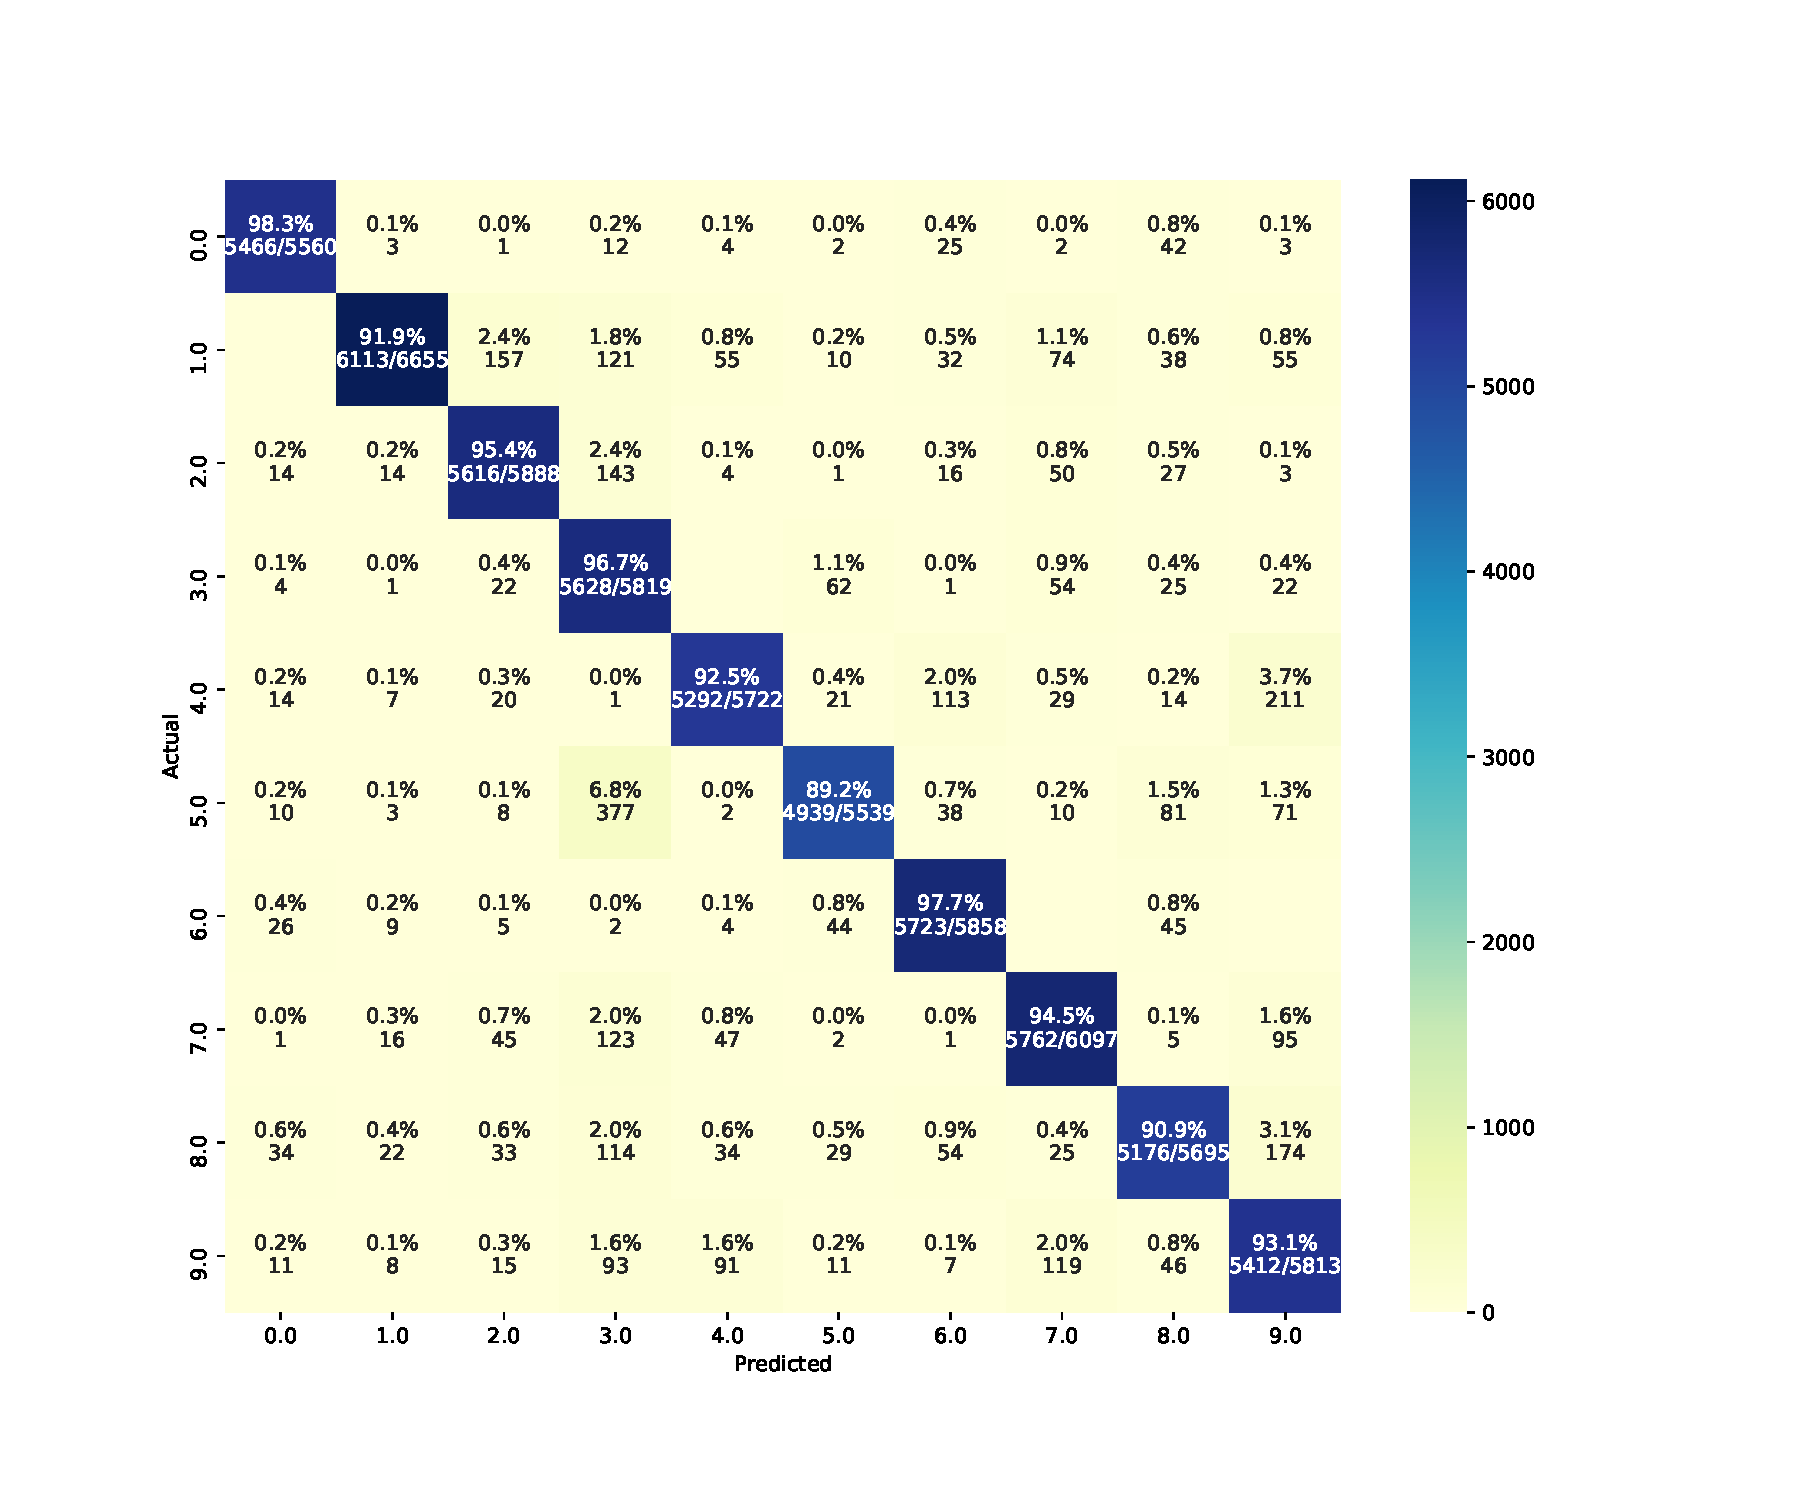
\includegraphics[width=1.1\textwidth]{confusion_knn.pdf}
    \caption{\label{fig:confusion_knn}Matriz de confusão do classificador kNN}
  \end{minipage}\hfill
  \begin{minipage}{.47\textwidth}
    \centering
    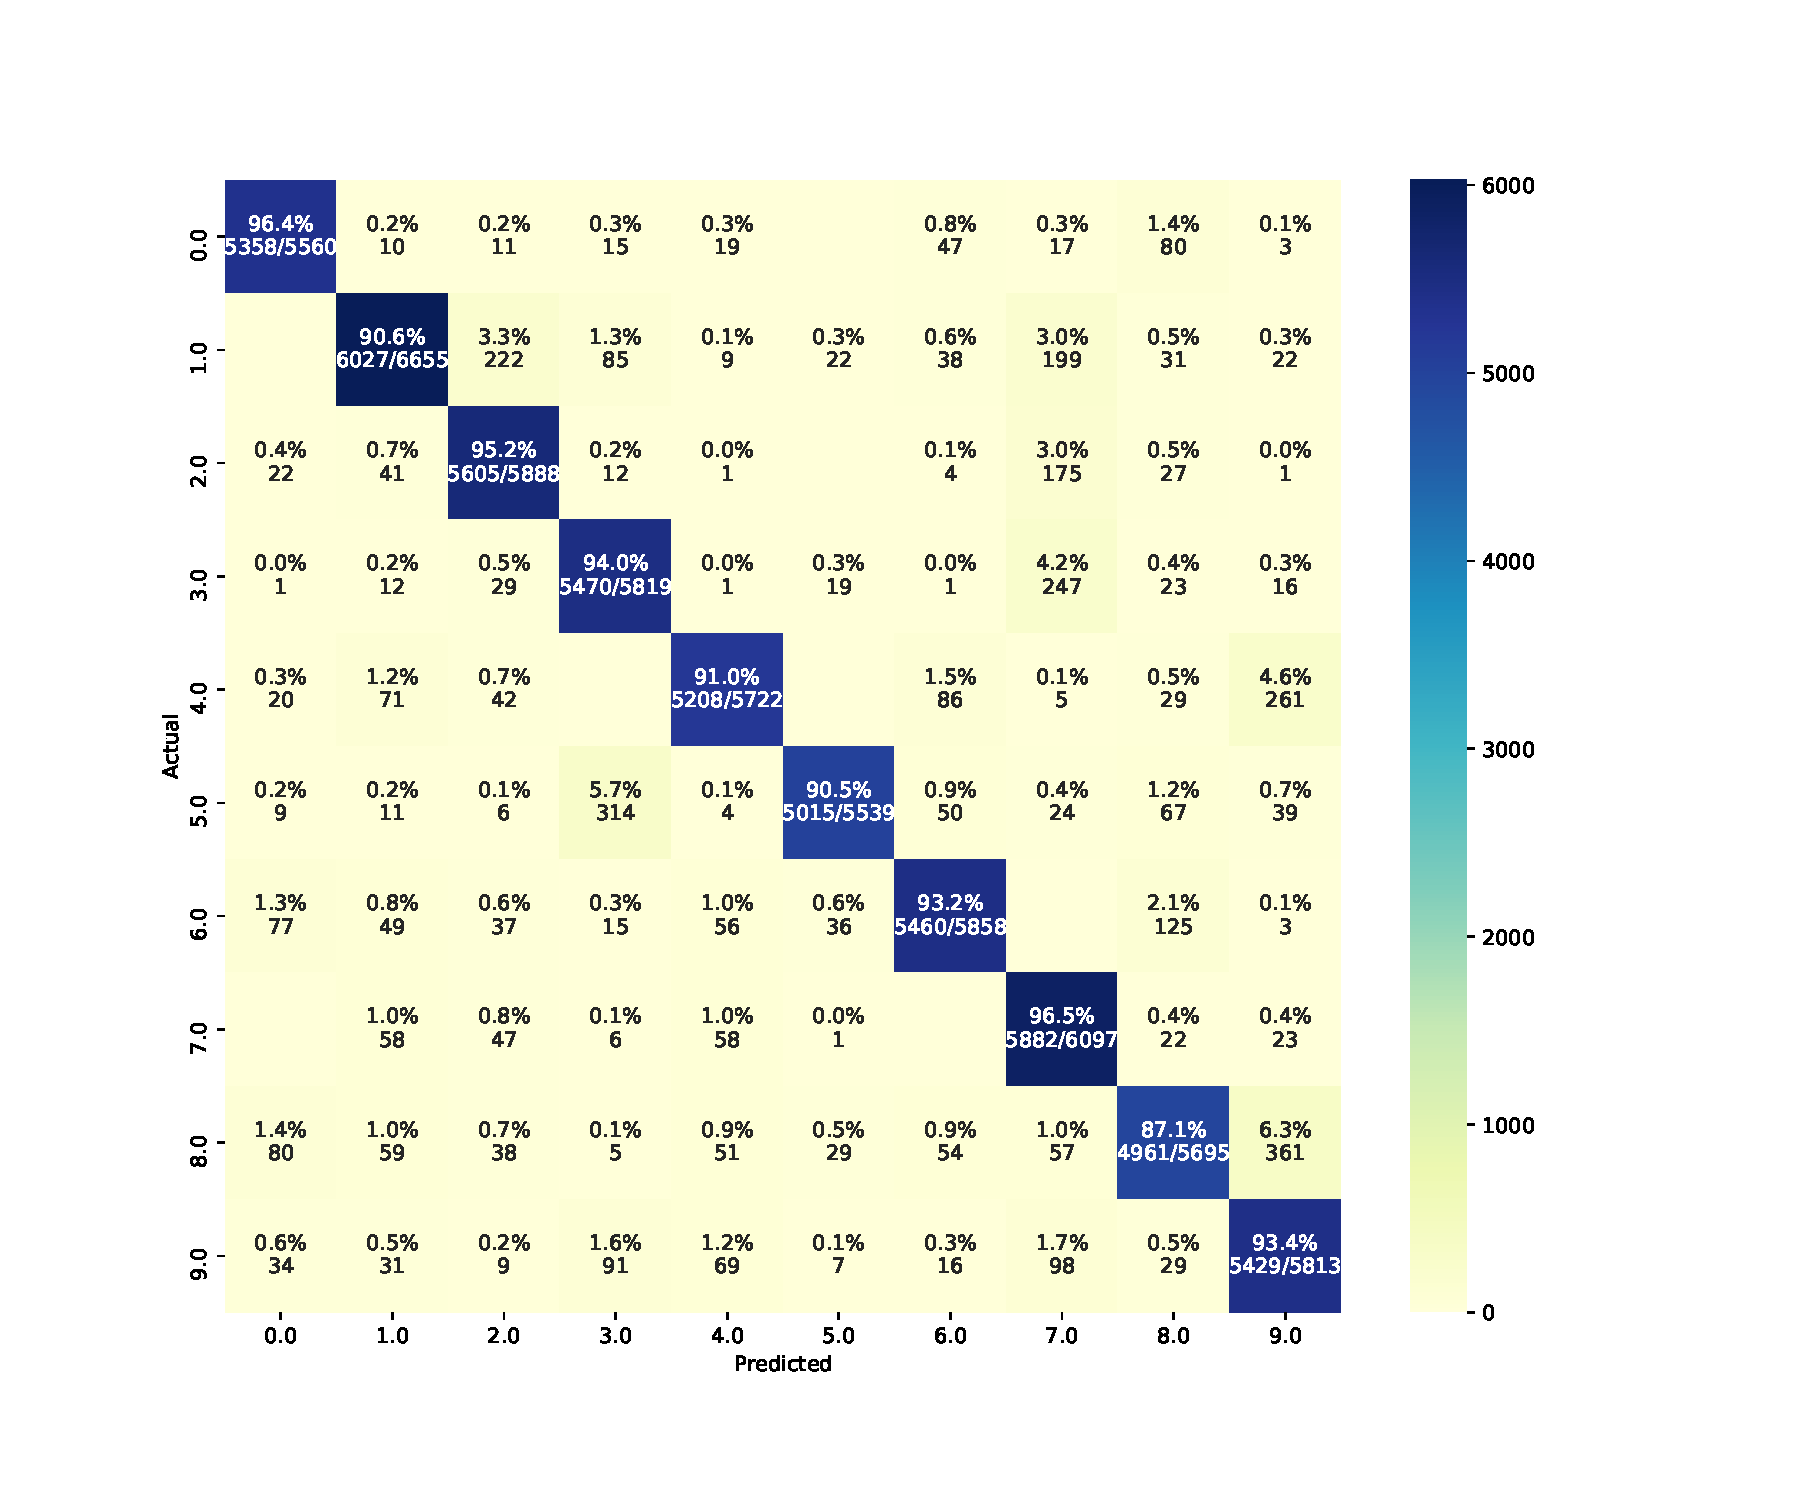
\includegraphics[width=1.1\textwidth]{confusion_lda.pdf}
    \caption{\label{fig:confusion_lda}Matriz de confusão do classificador LDA}
  \end{minipage}
\end{figure}

\begin{figure}[H]
\centering
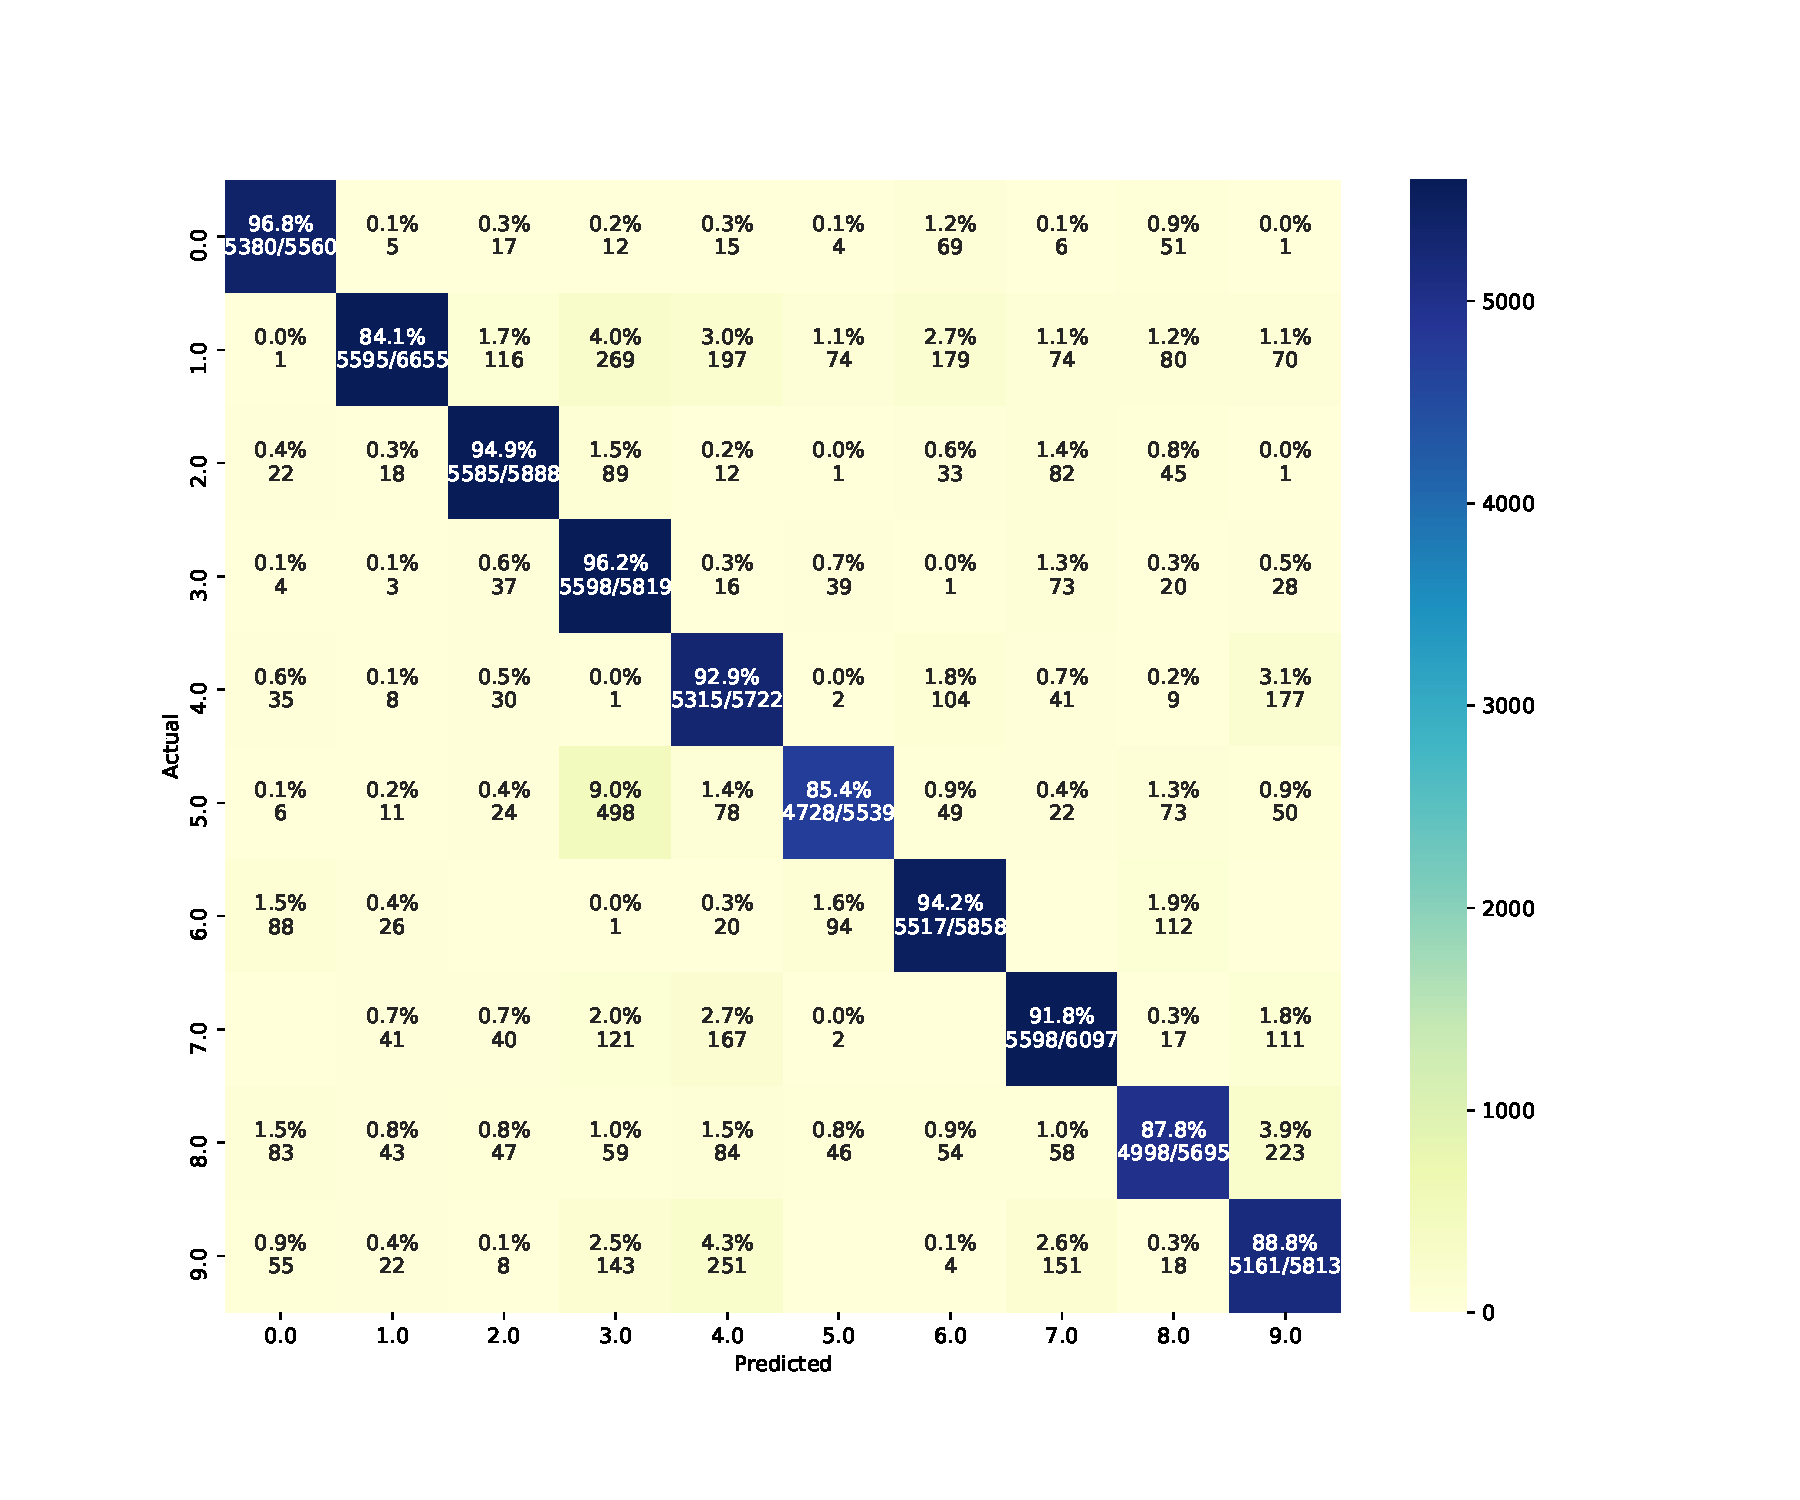
\includegraphics[width=0.8\textwidth]{confusion_logistic.pdf}
\caption{\label{fig:confusion_logistic}Matriz de confusão do classificador Logistic Regression}
\end{figure}

\begin{figure}[H]
\centering
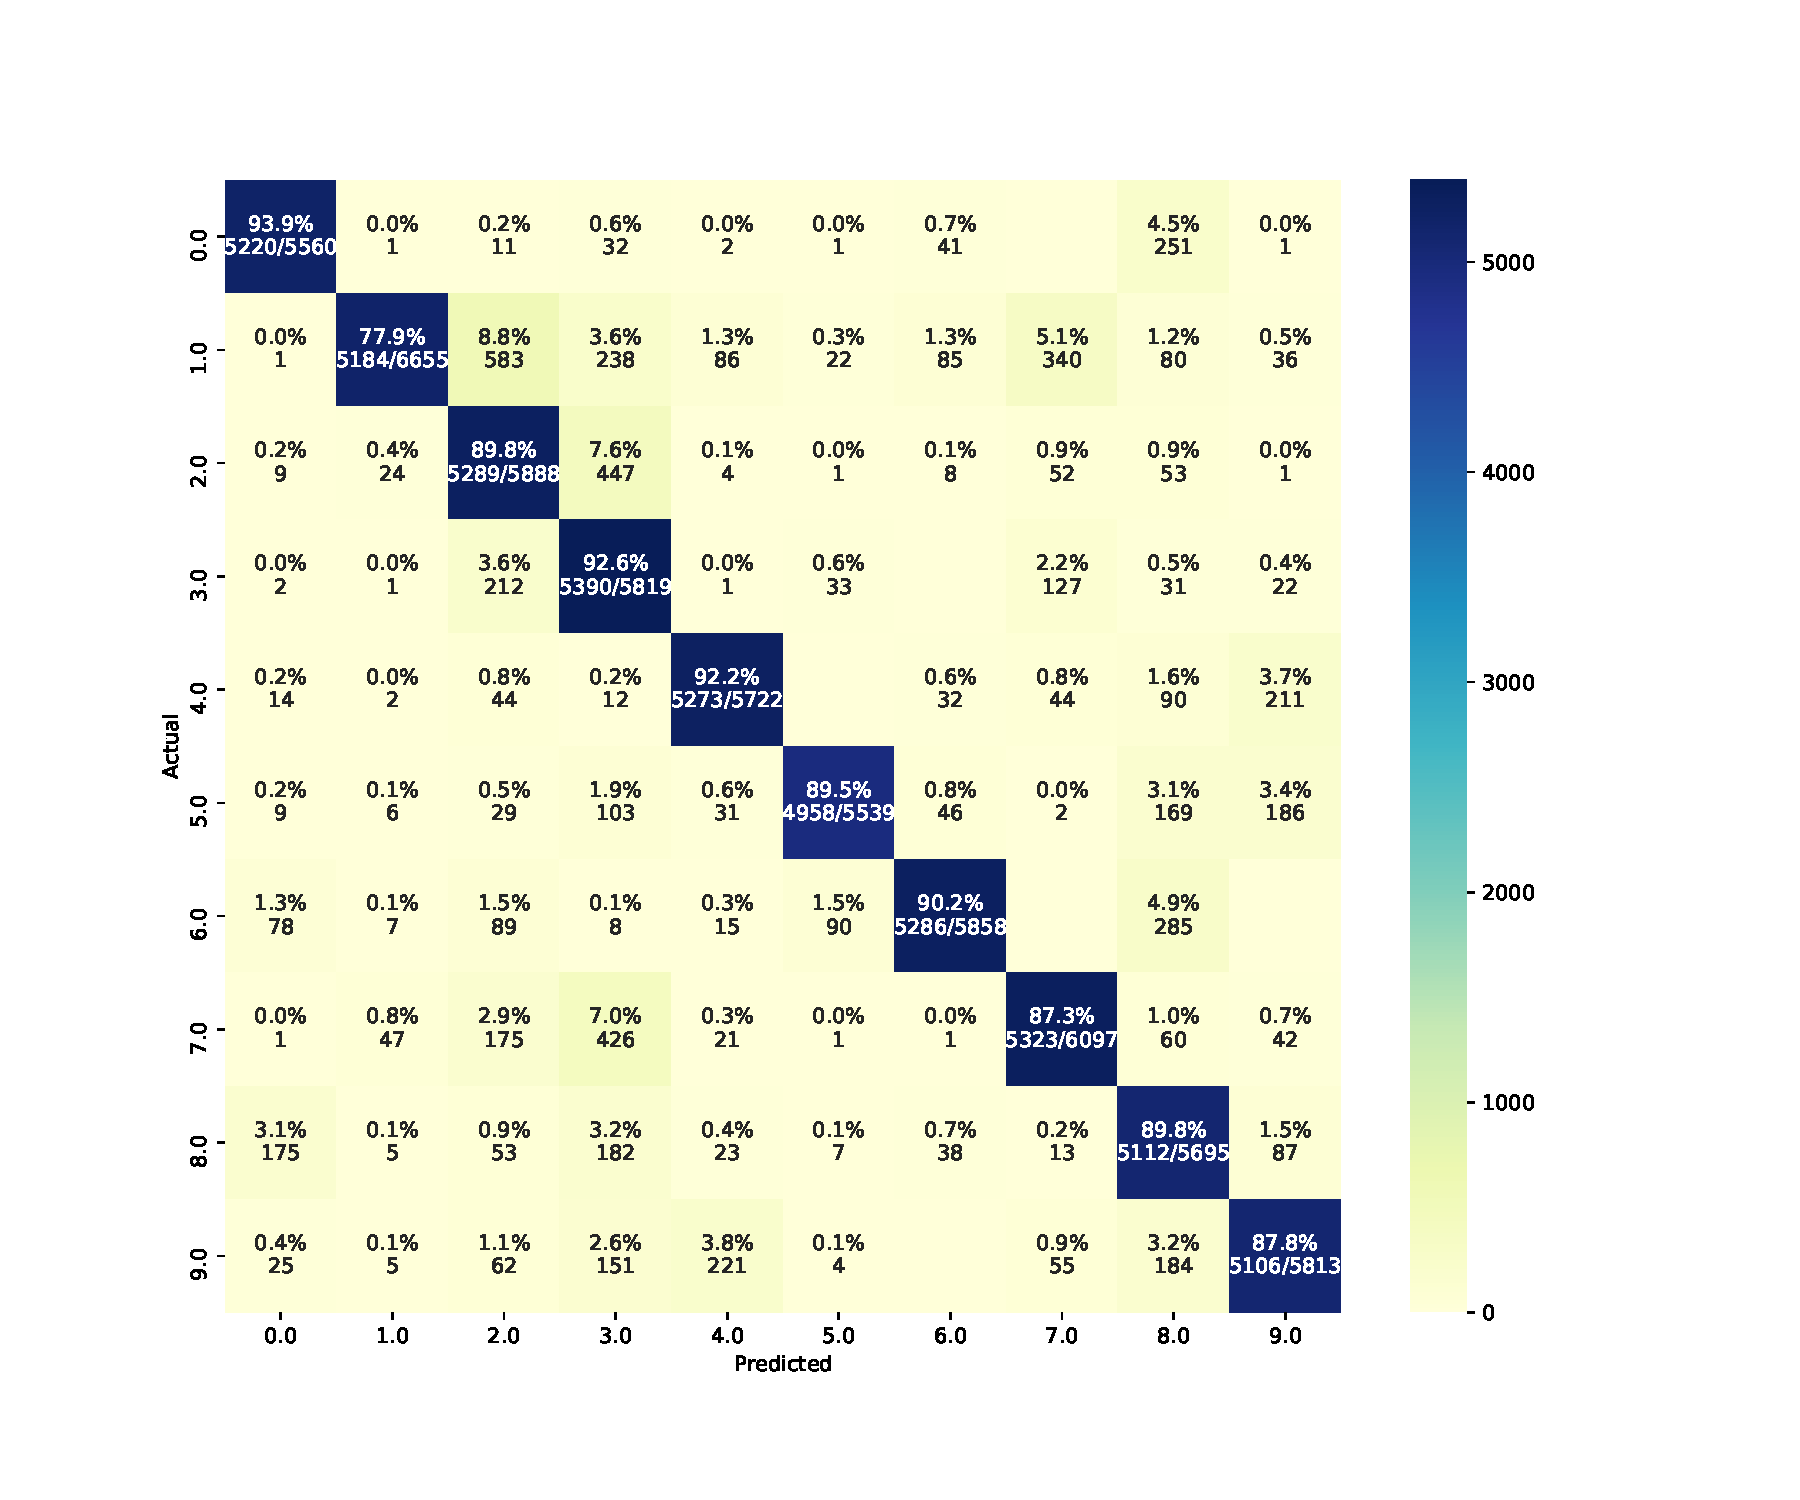
\includegraphics[width=0.8\textwidth]{confusion_naive.pdf}
\caption{\label{fig:confusion_naive}Matriz de confusão do classificador Naive Bayes}
\end{figure}

\begin{figure}[H]
\centering
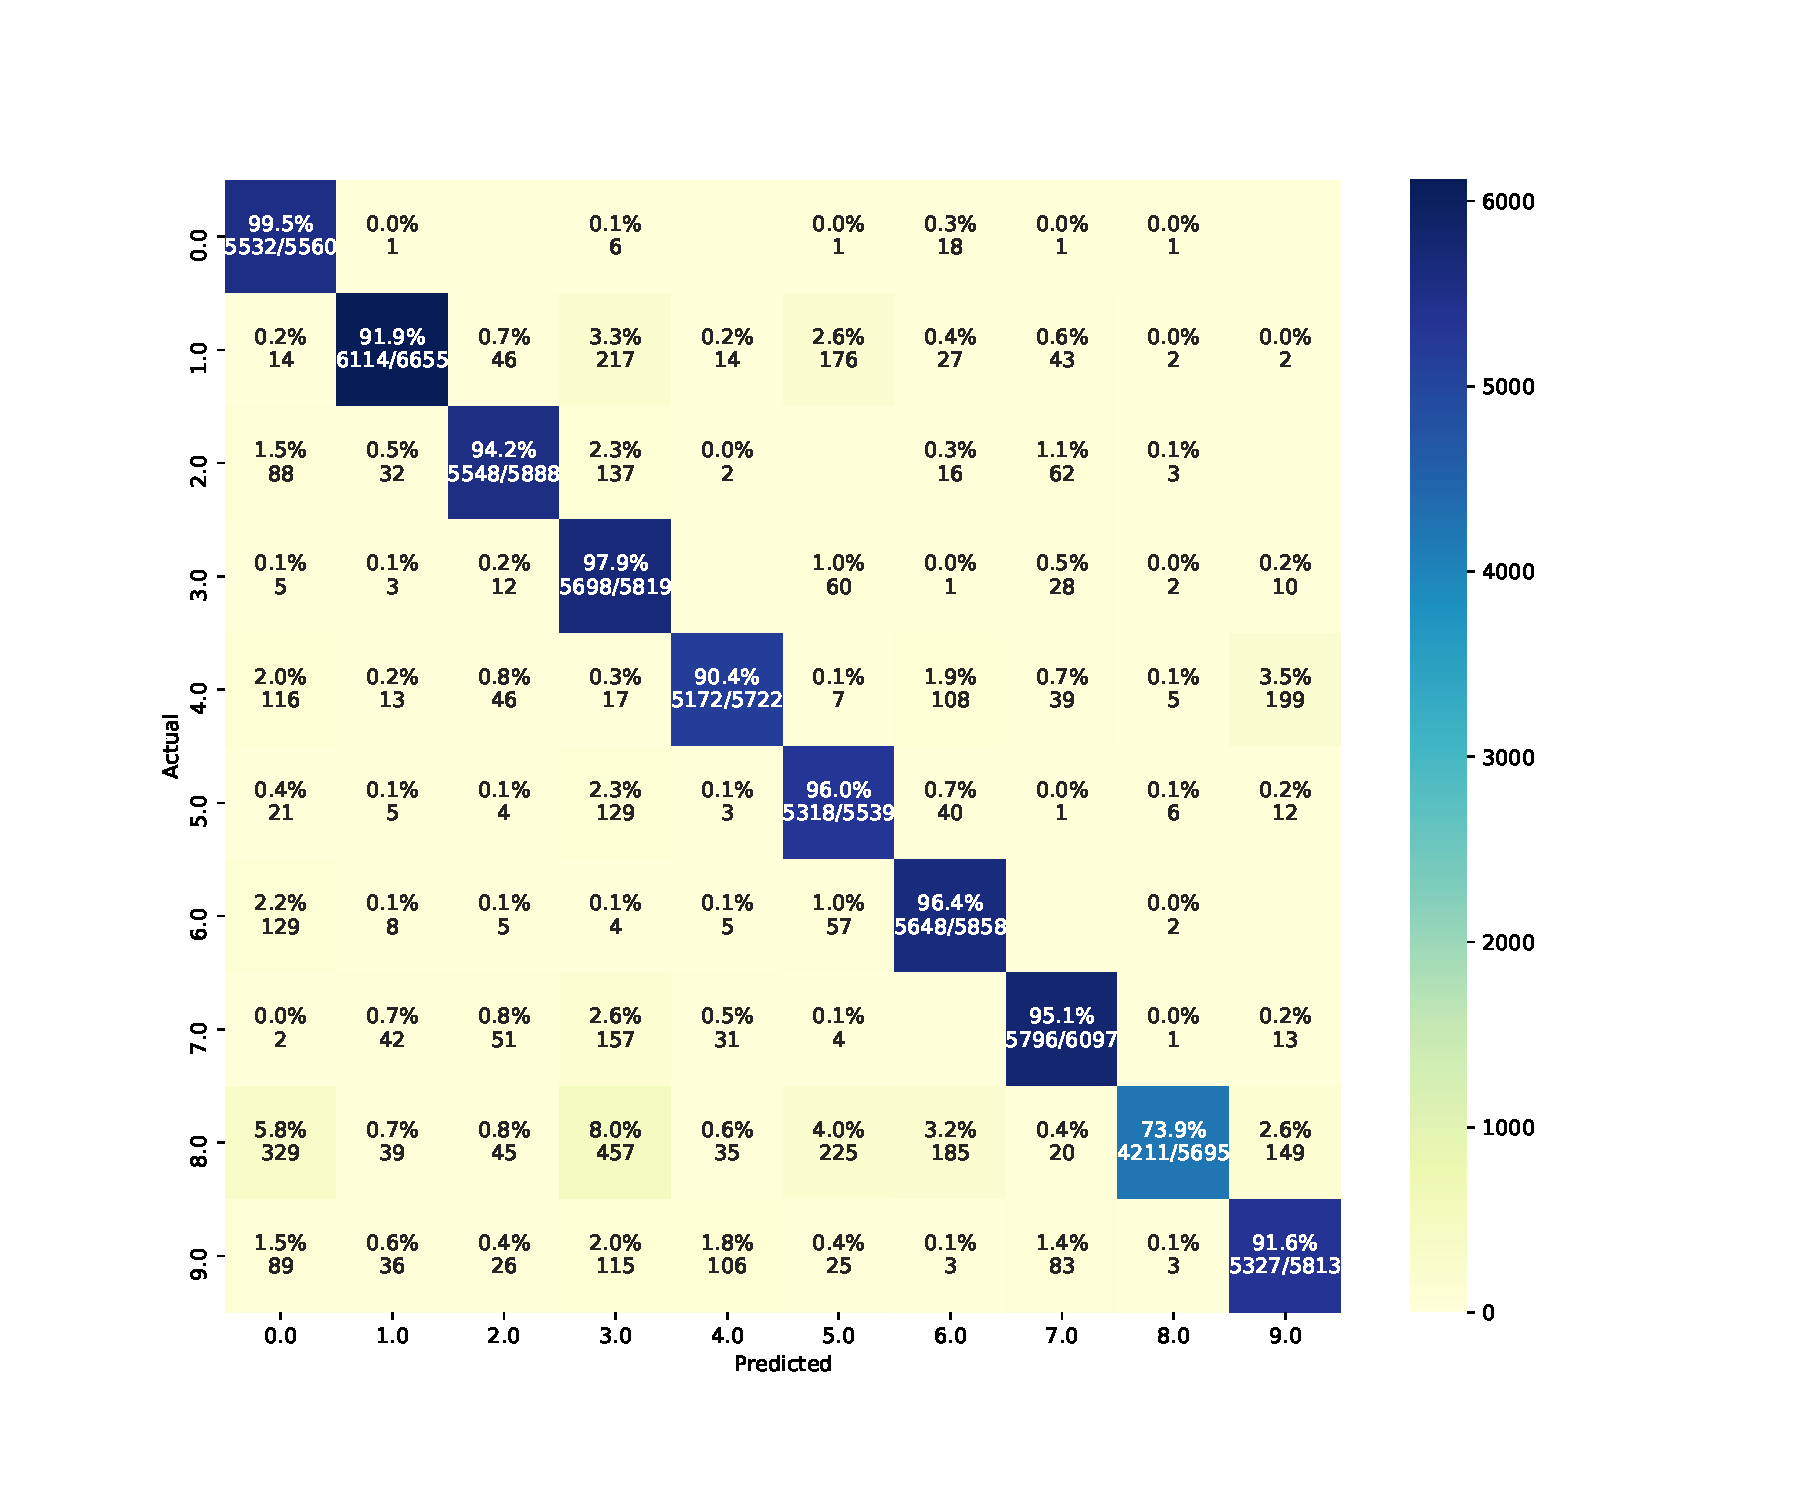
\includegraphics[width=0.8\textwidth]{confusion_perceptron.pdf}
\caption{\label{fig:confusion_perceptron}Matriz de confusão do classificador Perceptron}
\end{figure}

Teste \cite{greenwade93}.
